\chapter{Connection between URG and Other Canonical Transformations}
\label{urg_canonical}
\section{Poor man's scaling (PMS)}
\subsection{Formalism}
We first describe the formalism of the poor man's scaling (PMS) method, first formulated by Anderson \cite{Anderson}. The problem is defined as
\begin{equation}\begin{aligned}
	\label{problem}
\mathcal{H}\ket{\Psi} = E\ket{\Psi}
\end{aligned}\end{equation}
\(\mathcal{H}\) is the total Hamiltonian and \(\ket{\Psi}\) and \(E\) are the exact eigenstate and eigenvalue of \(\mathcal{H}\). We imagine a separation of the total Hilbert space into two set of states, and we call these two states \(\ket{0}\) and \(\ket{1}\). This separation depends on which scattering term we want to kill by this transformation. For example, in the URG, we typically select a particular electron \(q\beta\) and then kill the  scattering terms that change the number of this state. In that case, \(\ket{0}\) will refer to the set of states \(\left\{\ket{\hat n_{q\beta}=0}\otimes\ket{\phi_0}\right\}\) and \(\ket{1}\) will refer to the set of states \(\left\{\ket{\hat n_{q\beta}=1}\otimes\ket{\phi_1}\right\}\). \(\ket{\phi_{0,1}}\) refer to the states of all the other electrons. As another example, if we wanted to separate the charge-Kondo and the spin-Kondo from the SIAM, we would want to kill the terms that scatter between the spin-full subspace \(\hat n_d=1\) to the spin-less subspace \(\hat{n_d}=0,2\). These two will then be the \(\ket{0}\) and \(\ket{1}\) sets. 

Keeping this separation in mind, the exact eigenstate \(\ket{\Psi}\) can be split as 
\begin{equation}\begin{aligned}
\ket{\Psi} = \sum_i \ket{\phi_0^i} + \sum \ket{\phi_1^i}
\end{aligned}\end{equation}
The Hamiltonian can also be split as 
\begin{equation}\begin{aligned}
\mathcal{H} = H_0 + V_+ + V_-
\end{aligned}\end{equation}
\(H_0\) does not scatter between \(\left\{\ket{0}\right\}\) and \(\left\{\ket{1}\right\}\). It contains the diagonal parts as well as scatterings inside the subspaces. \(V_\pm\) scatter between the subspaces:
\begin{equation}\begin{aligned}
V_+ \left\{\ket{0}\right\} \mapsto \left\{\ket{1}\right\},&& V_+ \ket{1} \to 0\\
V_- \left\{\ket{1}\right\} \mapsto \left\{\ket{0}\right\},&& V_- \ket{0} \to 0
\end{aligned}\end{equation}
The Schrodinger equation can thus be split into
\begin{equation}\begin{aligned}
H_0 \sum_i \ket{\phi^i_0} + V_-\sum_i \ket{\phi^i_1} &= E \sum_i \ket{\phi^i_0}\\
H_0 \sum_i \ket{\phi^i_1} + V_+\sum_i \ket{\phi^i_0} &= E \sum_i \ket{\phi^i_1}\\
\end{aligned}\end{equation}
Eliminating \(\sum_i \ket{\phi^i_1}\) gives
\begin{equation}\begin{aligned}
H_0 \sum_i \ket{\phi^i_0} + V_-\frac{1}{E_1 - H_0}V_+\sum_i \ket{\phi^i_0} &= E \sum_i \ket{\phi^i_0}\\
\end{aligned}\end{equation}
The effective Hamiltonian in this subspace is therefore
\begin{equation}\begin{aligned}
	\tilde{\mathcal{H}}_0 = H_0 + V_-\frac{1}{E - H_0}V_+
\end{aligned}\end{equation}
Similarly, eliminating \(\sum_i \ket{\phi^i_0}\) gives the effective Hamiltonian in the other subspace,
\begin{equation}\begin{aligned}
	\tilde{\mathcal{H}}_1 = H_0 + V_+\frac{1}{E - H_0}V_-
\end{aligned}\end{equation}
The total effective Hamiltonian that does not scatter between the two subspaces is
\begin{equation}\begin{aligned}
	\tilde{\mathcal{H}}(E) = H_0 + \underbrace{V_-\frac{1}{E - H_0}V_+ +  V_+\frac{1}{E - H_0}V_-}_\text{renormalization}
\end{aligned}\end{equation}
This is of course a function of whatever exact energy eigenvalue we chose, \(E\). Different choices will give different effective Hamiltonians. The renormalization will now be written in terms of the matrix elements. Since the entire \(\mathcal{H}_X\) must be Hermitian, we must have \(V_- = V_+^\dagger \equiv V\).
\begin{equation}\begin{aligned}
\Delta \mathcal{H}(E) = V\frac{1}{E - H_0}V^\dagger +  V^\dagger\frac{1}{E - H_0}V
\end{aligned}\end{equation}
Now take the first term and insert complete bases on both sides of \(V\) and \(V^\dagger\).
\begin{equation}\begin{aligned}
V\frac{1}{E - H_0}V^\dagger &= \sum_{ijk}\ket{\phi_0^i}\bra{\phi_0^i}V\ket{\phi_1^j}\bra{\phi_1^j}\frac{1}{E - H_0}\ket{\phi_1^j}\bra{\phi_1^j}V^\dagger\ket{\phi_0^k}\bra{\phi_0^k} \\
                &= \sum_{ijk}\ket{\phi_0^i}V_{ij}\bra{\phi_1^j}\frac{1}{E - H_0}\ket{\phi_1^j}V^\dagger_{kj}\bra{\phi_0^k}\\
\end{aligned}\end{equation}
where we defined \(\bra{\phi_0^i}V\ket{\phi_1^j} = V_{ij}\). We now approximate \(H_0\) by keeping just the diagonal part, and allowing the balance to redefine \(E\) into \(\omega\). Then, \(\left(E - H_0\right) \ket{\phi_{0,1}^j} \equiv \left(\omega_{0,1} - E_{0,1}^j\right) \ket{\phi_{0,1}^j}\). That gives
\begin{equation}\begin{aligned}
\label{pms_dropV}
V\frac{1}{E - H_0}V^\dagger &= \sum_{ijk}\ket{\phi_0^i}\bra{\phi_0^k}\frac{V_{ij}V^\dagger_{kj}}{\omega_1 - E^j_1}
\end{aligned}\end{equation}
The second term similarly gives
\begin{equation}\begin{aligned}
V^\dagger\frac{1}{E - H_0}V = \sum_{ijk}\ket{\phi_1^i}\bra{\phi_1^k}\frac{V^\dagger_{ji}V_{jk}}{\omega_0 - E^j_0}
\end{aligned}\end{equation}
The total renormalization becomes
\begin{equation}\begin{aligned}
	\Delta \mathcal{H}(E) = \sum_{ijk}\left(\frac{1}{\omega_1 - E^j_1}\ket{\phi_0^i}\bra{\phi_0^k}V_{ij}V^\dagger_{kj} + \frac{1}{\omega_0 - E^j_0}\ket{\phi_1^i}\bra{\phi_1^k}V^\dagger_{ji}V_{jk}\right)
\end{aligned}\end{equation}
This is a general expression that would work irrespective of whether you are decoupling multiple electrons or a single electron. However, the \(\omega\) are unknown and we need some prescription for replacing them. Since the \(E\) is the eigenstate of the initial state on which the scattering terms act, it makes sense to replace them with the initial state energy.
\begin{equation}\begin{aligned}
	\Delta \mathcal{H}(E) = \sum_{ijk}\left(\frac{1}{E_0^k - E^j_1}\ket{\phi_0^i}\bra{\phi_0^k}V_{ij}V^\dagger_{kj} + \frac{1}{E_1^k - E^j_0}\ket{\phi_1^i}\bra{\phi_1^k}V^\dagger_{ji}V_{jk}\right)
\end{aligned}\end{equation}
However, closer inspection reveals that this choice makes the renormalization non-Hermitian. So the correct choice is to keep both the initial and final energies.
\begin{equation}\begin{aligned}
	\Delta \mathcal{H} &= \frac{1}{2}\sum_{ijk}\frac{1}{\omega_1 - E^j_1}\left(\ket{\phi_0^i}\bra{\phi_0^k}V_{ij}V^\dagger_{kj} + \ket{\phi_0^k}\bra{\phi_0^i}V_{kj}V^\dagger_{ij}\right)\\
			   &+\frac{1}{2}\sum_{ijk}\frac{1}{\omega_0 - E^j_0}\left(\ket{\phi_1^i}\bra{\phi_1^k}V^\dagger_{ji}V_{jk} + \ket{\phi_1^k}\bra{\phi_1^i}V^\dagger_{jk}V_{ji}\right)\\
			   &= \frac{1}{2}\sum_{ijk}\left(\frac{1}{E_0^k - E^j_1}\ket{\phi_0^i}\bra{\phi_0^k}V_{ij}V^\dagger_{kj} + \frac{1}{E_0^k - E^j_1}\ket{\phi_0^k}\bra{\phi_0^i}V_{kj}V^\dagger_{ij}\right)\\
			   &+\frac{1}{2}\sum_{ijk}\left(\frac{1}{E_1^k - E^j_0}\ket{\phi_1^i}\bra{\phi_1^k}V^\dagger_{ji}V_{jk} + \frac{1}{E_1^k - E^j_0}\ket{\phi_1^k}\bra{\phi_1^i}V^\dagger_{jk}V_{ji}\right)
\end{aligned}\end{equation}
Therefore,
\begin{equation}\begin{aligned}
	\label{pmsren}
	\Delta \mathcal{H} &= \frac{1}{2}\sum_{ijk}\left(\frac{1}{E_0^k - E^j_1} + \frac{1}{E_0^i - E^j_1}\right)\ket{\phi_0^i}\bra{\phi_0^k}V_{ij}V^\dagger_{kj}\\
			   &+\frac{1}{2}\sum_{ijk}\left(\frac{1}{E_1^k - E^j_0}+ \frac{1}{E_1^i - E^j_0}\right)\ket{\phi_1^i}\bra{\phi_1^k}V^\dagger_{ji}V_{jk}\\
\end{aligned}\end{equation}
In summary, the prescription of replacing all \(\omega\) with the initial state energy will be correct only if the initial and final states are the same. This happens when we are decoupling a single-electron state - then the total renormalization is of the form \(c^\dagger T^\dagger c\) such that we start from an initial state, scatter to an intermediate state and then go back to the initial state so that the final state is the same as the initial state. However, if we are using PMS to decouple states in one-shot, each subspace will have multiple states and there might be terms where we do not end up at the initial state we started with. Then the correct prescription would be to use the mean of the initial and final state denominators.

One might wonder how we can generate higher order terms in this method. Eq.~\ref{pmsren}, as it stands, has only \(\mathcal{O}(V^2)\) terms. The higher order terms were actually dropped when we replaced \(H_0\) with its diagonal part in eq.~\ref{pms_dropV}. To see the higher order term, we do not drop the off-diagonal part in the denominator, but split the total \(H_0\) into a diagonal and an off-diagonal part: \(H_0 = H_d + X\). Note that \(X\) is off-diagonal in the subspace of the states that have not been decoupled yet but will be decoupled later. They represent scattering between the lower energy states. \(X\) is still diagonal with respect to the states that we \text{are} decoupling presently. The total effective Hamiltonian becomes
\begin{equation}\begin{aligned}
	\tilde{\mathcal{H}}(E) = H_0 + V\frac{1}{G_0(E)^{-1} - X}V^\dagger +  V^\dagger\frac{1}{G_0(E)^{-1} - X}V
\end{aligned}\end{equation}
where \(G_0(E)^{-1} = E - H_d\) is the inverse of the non-interacting Greens function. To allow computation, we can expand the denominator in powers of \(XG_0(E)^{-1}\):
\begin{equation}\begin{aligned}
	\label{pms_third}
	\Delta H \equiv \tilde{\mathcal{H}}(E) - H_0 =& VG_0(E)\left[1 + XG_0(E) + XG_0(E)XG_0(E) + ...\right] V^\dagger +  V^\dagger\frac{1}{G_0(E)^{-1} - X}V\\
	=& \underbrace{V G_0(E) V^\dagger + V^\dagger G_0(E) V}_\text{two vertex or one loop correction} + \underbrace{VG_0(E)XG_0(E)V^\dagger + V^\dagger G_0(E)XG_0(E)V}_\text{three vertex or two loop correction} \\
			       &+ \text{higher loop corrections}
\end{aligned}\end{equation}
\subsection{PMS third order equations for symmetric multi-channel Kondo model}
To get a clear idea of what the various terms in eq.~\ref{pms_third} mean, we will calculate the multi-channel Kondo model RG equations up to third order. The model is
\begin{equation}\begin{aligned}
	H = \sum_{k\sigma,\gamma}\epsilon_{k\sigma}^{(\gamma)}c^\dagger_{k\sigma}c^{(\gamma)}_{k\sigma} + \sum_{k\alpha,k^\prime \alpha^\prime,\gamma,a}J^a S_d^a \sigma^a_{\alpha\alpha^\prime}{c^{(\gamma)}_{k\alpha}}^\dagger c^{(\gamma)}_{k^\prime\alpha^\prime}
\end{aligned}\end{equation}
\(a\) goes over \(x,y,z\) and represents the directions. \(S_d^a\) therefore represents the spin operators for the impurity along the \(x,y\) and \(z\) directions. The labels \(k\alpha\) and \(k^\prime\alpha^\prime\) sum over the conduction electrons, while the index \(\gamma\) represents the channel. We will first calculate the second order terms. The virtual particle term is
\begin{equation}\begin{aligned}
	V G_0(E) V^\dagger = \sum_{k,k^\prime,\alpha,\alpha^\prime,q,\beta,\gamma,a,b}{c^{(\gamma)}_{q\beta}}^\dagger {c^{(\gamma)}_{k\alpha}} S_d^a \sigma^a_{\beta\alpha} \frac{J^a J^b}{E - H_d} {c^{(\gamma)}_{k^\prime\alpha^\prime}}^\dagger {c^{(\gamma)}_{q\beta}}S_d^b \sigma^b_{\alpha^\prime\beta}
\end{aligned}\end{equation}
The label \(q\) sums over the momentum states being decoupled \(\left( |\epsilon_q| \in \left[D-|\delta D|, D\right]  \right) \). The labels \(k,k^\prime\), on the other hand, sum over the momentum states that are not being decoupled, so they lie in the complimentary range. The denominator of the Greens function is the excitation energy \(\epsilon_q - \epsilon_{k^\prime}\). We will now simplify the term.
\begin{equation}\begin{aligned}
	V G_0(E) V^\dagger &= \sum_{k,k^\prime,\alpha,\alpha^\prime,q,\beta,\gamma, a,b} \frac{J^a J^b}{\epsilon_q - \epsilon_{k^\prime}}S_d^a \sigma^a_{\beta\alpha} S_d^b \sigma^b_{\alpha^\prime\beta}{c^{(\gamma)}_{q\beta}}^\dagger {c^{(\gamma)}_{k\alpha}} {c^{(\gamma)}_{k^\prime\alpha^\prime}}^\dagger {c^{(\gamma)}_{q\beta}}\\
			   &= \sum_{k,k^\prime,\alpha,\alpha^\prime,\beta,\gamma, a,b} \frac{J^a J^b}{\epsilon_q - \epsilon_{k^\prime}}S_d^a \sigma^a_{\beta\alpha} S_d^b \sigma^b_{\alpha^\prime\beta} {c^{(\gamma)}_{k\alpha}} {c^{(\gamma)}_{k^\prime\alpha^\prime}}^\dagger \sum_q {\hat n^{(\gamma)}_{q\beta}}\\
			   &= \sum_{k,k^\prime,\alpha,\alpha^\prime,\beta,\gamma, a,b} S_d^a \sigma^a_{\beta\alpha} S_d^b \sigma^b_{\alpha^\prime\beta} {c^{(\gamma)}_{k\alpha}} {c^{(\gamma)}_{k^\prime\alpha^\prime}}^\dagger \int_{-D}^{-D + |\delta D|} d\epsilon \rho(\epsilon) \frac{J^a J^b {\hat n^{(\gamma)}(\epsilon)_{\beta}}}{\epsilon_q - \epsilon_{k^\prime}}\\
			   &= \sum_{k,k^\prime,\alpha,\alpha^\prime,\beta,\gamma, a,b} S_d^a \sigma^a_{\beta\alpha} S_d^b \sigma^b_{\alpha^\prime\beta} {c^{(\gamma)}_{k\alpha}} {c^{(\gamma)}_{k^\prime\alpha^\prime}}^\dagger \frac{J^a J^b \rho(0) |\delta D|}{-D} ~~~\left[\hat n(\epsilon) = \theta(-\epsilon), |\epsilon_{k^\prime}| \ll D\right] \\
			   &= \sum_{\alpha,\alpha^\prime,a,b} S_d^a S_d^b \left(\sigma^b \sigma^a\right)_{\alpha^\prime,\alpha} \sum_{k,k^\prime,\gamma}{c^{(\gamma)}_{k\alpha}} {c^{(\gamma)}_{k^\prime\alpha^\prime}}^\dagger \frac{J^a J^b \rho(0) |\delta D|}{-D} \\
			   &= \sum_{\alpha,\alpha^\prime,a,b} \left(\frac{1}{4}\delta_{ab} + \frac{i}{2}\sum_c \epsilon^{abc}S_d^c\right) \left(\delta_{ab} + i\sum_c \epsilon^{bac}\sigma^c\right)_{\alpha^\prime,\alpha} \sum_{k,k^\prime,\gamma}{c^{(\gamma)}_{k\alpha}} {c^{(\gamma)}_{k^\prime\alpha^\prime}}^\dagger \frac{J^a J^b \rho(0) |\delta D|}{-D} \\
\end{aligned}\end{equation}
The spin part can now be simplified:
\begin{equation}\begin{aligned}
	\sum_{a,b} J^a J^b \left(\frac{1}{4}\delta_{ab} + \frac{i}{2}\sum_c \epsilon^{abc}S_d^c\right) \left(\delta_{ab} + i\sum_c \epsilon^{bac}\sigma^c\right)_{\alpha^\prime,\alpha} = \frac{\sum_a {J^a}^2}{4} \delta_{\alpha,\alpha^\prime} + \frac{1}{2}\sum_{a,b,c,c^\prime}J^a J^b \epsilon^{abc}\epsilon^{abc^\prime}S_d^c \left(\sigma^c\right)_{\alpha^\prime\alpha}\\
	= \frac{\sum_a {J^a}^2}{4} \delta_{\alpha,\alpha^\prime} + \frac{1}{2}\sum_c S_d^c \sigma^c_{\alpha^\prime\alpha}\left(\sum_{a,b,\atop{a\neq b}}J^a J^b - 2 J^c\sum_{a \atop{a \neq c}}J^a\right)
\end{aligned}\end{equation}
The constant part renormalizes a potential scattering, so we drop that part. The renormalization from the other part is
\begin{equation}\begin{aligned}
	\sum_{\alpha,\alpha^\prime,c} S_d^c \sigma^c_{\alpha^\prime\alpha} \sum_{k,k^\prime,\gamma}{c^{(\gamma)}_{k\alpha}} {c^{(\gamma)}_{k^\prime\alpha^\prime}}^\dagger \frac{\frac{1}{2}\left(\sum_{a,b,\atop{a\neq b}}J^a J^b - 2 J^c\sum_{a \atop{a \neq c}}J^a\right)\rho(0) |\delta D|}{-D}\\
	= \sum_{\alpha,\alpha^\prime,c} S_d^c \sigma^c_{\alpha^\prime\alpha} \sum_{k,k^\prime,\gamma}{c^{(\gamma)}_{k^\prime\alpha^\prime}}^\dagger {c^{(\gamma)}_{k\alpha}} \frac{\frac{1}{2}\left(\sum_{a,b,\atop{a\neq b}}J^a J^b - 2 J^c\sum_{a \atop{a \neq c}}J^a\right)\rho(0) |\delta D|}{D}
\end{aligned}\end{equation}
The virtual hole term \(V^\dagger G_0(E) V\) gives the same contribution. The total renormalization at second order is therefore
\begin{equation}\begin{aligned}
	\delta J^c = \frac{\left(\sum_{a,b,\atop{a\neq b}}J^a J^b - 2 J^c\sum_{a \atop{a \neq c}}J^a\right)\rho(0) |\delta D|}{D} = \frac{2J^{c+1}J^{c-1}\rho(0) |\delta D|}{D}
\end{aligned}\end{equation}
where \(\left\{c-1,c,c+1\right\}\) is a cyclic permutation of \(\left\{ x,y,z \right\} \). This reveals that the anisotropic Kondo coupling RG equations have a cyclic form:
\begin{equation}\begin{aligned}
	\delta J^x = \frac{2J^y J^z\rho(0) |\delta D|}{D}
\end{aligned}\end{equation}
Cyclic permutations of the labels \(x,y,z\) produce the other equations. From here on, we will assume \(J^a = J\) for simplicity. This gives, at second order,
\begin{equation}\begin{aligned}
	\delta J = \frac{2J^2\rho(0) |\delta D|}{D}
\end{aligned}\end{equation}

We now consider the third order term. The virtual hole three vertex term, \(V^\dagger G_0(E)XG_0(E)V\), is of the form
\begin{equation}\begin{aligned}
	J^3\sum_{q,k_1,k_2,k,k^\prime,\atop{\alpha,\alpha^\prime,\alpha_1,\alpha_2,\beta,\atop{\gamma_1,\gamma_2}}}{c^{(\gamma_1)}_{q\beta}}^\dagger {c^{(\gamma_1)}_{k\alpha}}\vec{S_d}\cdot\vec{\sigma}_{\beta \alpha} \frac{1}{E - H_d} {c^{(\gamma_2)}_{k_1 \alpha_1}}^\dagger c_{k_2 \alpha_2}^{(\gamma_2)}\vec{S_d}\cdot\vec{\sigma}_{\alpha_1 \alpha_2} \frac{1}{E - H_d} {c^{(\gamma_1)}_{k^\prime\alpha^\prime}}^\dagger {c^{(\gamma_1)}_{q\beta}}\vec{S_d}\cdot\vec{\sigma}_{\alpha^\prime \beta}
\end{aligned}\end{equation}
The other term among the two third order terms is the virtual particle term. The labels \(q,k,k^\prime,k_1,k_2\) run over the momentum states, \(\alpha,\alpha^\prime,\alpha_1,\alpha_2,\beta\) run over the spin indices and \(\gamma_1,\gamma_2\) run over the channel indices. \(q,\beta\) are the labels of the momentum states that are being decoupled. \(|\epsilon_q|\) therefore lies in the range \(\left[D, D - \delta D\right] \). The rest of the labels \((k,\alpha),(k_1,\alpha_1),(k_2,\alpha_2)\) lie in the compliment range and represent electrons that are not being decoupled at this step.

The denominator of the right-most Greens function measures the energy difference between the initial state and the state reached after the first excitation. This difference is \(\epsilon_q - \epsilon_{k^\prime}\). Similarly, the second Greens function has the energy difference between the initial state and the one obtained after two subsequent excitations. This difference is \(\epsilon_q - \epsilon_{k^\prime} + \epsilon_{k_2} - \epsilon_{k_1}\). With this substitution, we get 
\begin{equation}\begin{aligned}
	V^\dagger G_0(E)XG_0(E)V = J^3\sum_{q,k_1,k_2,k,k^\prime,\atop{\alpha,\alpha^\prime,\alpha_1,\alpha_2,\beta,\atop{\gamma_1,\gamma_2}}}\frac{{c^{(\gamma_1)}_{q\beta}}^\dagger {c^{(\gamma_1)}_{k\alpha}}\vec{S_d}\cdot\vec{\sigma}_{\beta \alpha} {c^{(\gamma_2)}_{k_1 \alpha_1}}^\dagger{c^{(\gamma_2)}_{k_2 \alpha_2}}\vec{S_d}\cdot\vec{\sigma}_{\alpha_1 \alpha_2} {c^{(\gamma_1)}_{k^\prime\alpha^\prime}}^\dagger {c^{(\gamma_1)}_{q\beta}}\vec{S_d}\cdot\vec{\sigma}_{\alpha \beta}}{\left(\epsilon_q - \epsilon_{k^\prime} + \epsilon_{k_2} - \epsilon_{k_1}\right)\left(\epsilon_q - \epsilon_{k^\prime}\right)}
\end{aligned}\end{equation}
The sum over \(q\) can be performed in the usual manner.
\begin{equation}\begin{aligned}
	\sum_q \frac{c^\dagger_{q\beta}c_{q\beta}}{\left(\epsilon_q - \epsilon_{k^\prime} + \epsilon_{k_2} - \epsilon_{k_1}\right)\left(\epsilon_q - \epsilon_{k^\prime}\right)} = \int_{-D}^{-D + |\delta D|} \frac{d\epsilon \rho(\epsilon)\hat n(\epsilon)}{\left(\epsilon - \epsilon_{k^\prime} + \epsilon_{k_2} - \epsilon_{k_1}\right)\left(\epsilon - \epsilon_{k^\prime}\right) }\\
	= \frac{\rho(0) |\delta D|}{\left(D + \epsilon_{k^\prime} - \epsilon_{k_2} + \epsilon_{k_1}\right)\left(D + \epsilon_{k^\prime}\right)}
\end{aligned}\end{equation}
where we have taken \(\rho(\epsilon) = \rho(0)\), \(\hat n(\epsilon) = \theta(-\epsilon)\) and \(\epsilon_q \simeq -D\). 

For the next step, note that \(\vec{S_d}\cdot\vec{\sigma}_{x,y} = \sum_{a}S_d^a \sigma^a_{x,y}\). Substituting this into \(V^\dagger G_0(E)XG_0(E)V\) gives
\begin{equation}\begin{aligned}
	&\sum_{\gamma_1,\gamma_2}\sum_{k_1,k_2,k,k^\prime}\sum_{\alpha,\alpha^\prime,\alpha_1,\alpha_2,\beta} \sum_{a,b,c}\frac{J^3\rho(0) |\delta D|}{\left(D + \epsilon_{k^\prime} - \epsilon_{k_2} + \epsilon_{k_1}\right)\left(D + \epsilon_{k^\prime}\right)} S_d^a\sigma^a_{\beta \alpha}S_d^b\sigma^b_{\alpha_1 \alpha_2}S_d^c \sigma^c_{\alpha^\prime \beta} c^{(\gamma_1)}_{k\alpha}{c^{(\gamma_2)}_{k_1 \alpha_1}}^\dagger c^{(\gamma_2)}_{k_2 \alpha_2} {c^{(\gamma_1)}_{k^\prime\alpha^\prime}}^\dagger
\end{aligned}\end{equation}
Now, note that all not all combinations of the momenta will renormalize the \(\vec{S_d}\cdot\vec{s}\) term of the Hamiltonian. In order for such a term to come out, the four remaining momenta must be contracted to two. The first set of terms that satisfy this requirement is given by the condition  \(k^\prime\alpha^\prime = k\alpha\). The renormalization from this subset of terms is
\begin{equation}\begin{aligned}
&\sum_{\gamma_1,\gamma_2}\sum_{k_1,k_2,k}\sum_{\alpha,\alpha_1,\alpha_2,\beta} \sum_{a,b,c}\frac{J^3\rho(0) |\delta D|}{\left(D + \epsilon_k - \epsilon_{k_2} + \epsilon_{k_1}\right)\left(D + \epsilon_k\right)} S_d^a\sigma^a_{\beta \alpha}S_d^b\sigma^b_{\alpha_1 \alpha_2}S_d^c \sigma^c_{\alpha \beta} {c^{(\gamma_2)}_{k_1 \alpha_1}}^\dagger c^{(\gamma_2)}_{k_2 \alpha_2}c^{(\gamma_1)}_{k\alpha}{c^{(\gamma_1)}_{k\alpha}}^\dagger \\
&=\sum_{\gamma_2}\sum_{k_1,k_2}\sum_{\alpha,\alpha_1,\alpha_2,\beta} \sum_{a,b,c} J^3\rho(0) |\delta D| S_d^a\sigma^a_{\beta \alpha}S_d^b\sigma^b_{\alpha_1 \alpha_2}S_d^c\sigma^c_{\alpha \beta}{c^{(\gamma_2)}_{k_1 \alpha_1}}^\dagger c^{(\gamma_2)}_{k_2 \alpha_2} \sum_{\gamma_1}\int_{0}^{D - |\delta D|}\frac{ d\epsilon\rho(\epsilon) }{\left(D + \epsilon - \epsilon_{k_2} + \epsilon_{k_1}\right)\left(D + \epsilon\right)}\\
&\simeq\sum_{\gamma_2}\sum_{k_1,k_2}\sum_{\alpha,\alpha_1,\alpha_2,\beta} \sum_{a,b,c} J^3\rho(0) |\delta D| S_d^a\sigma^a_{\beta \alpha}S_d^b\sigma^b_{\alpha_1 \alpha_2}S_d^c\sigma^c_{\alpha \beta}{c^{(\gamma_2)}_{k_1 \alpha_1}}^\dagger c^{(\gamma_2)}_{k_2 \alpha_2} \sum_{\gamma_1}\int_{0}^{D - |\delta D|}\frac{ d\epsilon\rho(\epsilon) }{\left(D + \epsilon\right)^2}\\
&=\frac{K \rho^2(0) J^3|\delta D|}{2D} \sum_{\alpha,\beta} \sum_{a,c,b}\sum_{\alpha_1,\alpha_2}S_d^a S_d^b S_d^c\sigma^a_{\beta \alpha} \sigma^b_{\alpha_1 \alpha_2} \sigma^c_{\alpha \beta} \sum_{k_1,k_2,\gamma_2}{c^{(\gamma_2)}_{k_1 \alpha_1}}^\dagger c^{(\gamma_2)}_{k_2 \alpha_2}~.\\
\end{aligned}\end{equation}
\(K = \sum_{\gamma_1}\) is the total number of channels. The other set of terms is given by the condition \(k_1\alpha_1 = k_2\alpha_2\). The renormalization from these terms can be calculated similarly:
\begin{equation}\begin{aligned}
	&\sum_{\gamma_1,\gamma_2}\sum_{k_1,k,k^\prime}\sum_{\alpha,\alpha^\prime,\alpha_1,\beta} \sum_{a,b,c}\frac{J^3 \rho(0) |\delta D|}{\left(D + \epsilon_{k^\prime}\right)^2} S_d^a\sigma^a_{\beta \alpha}S_d^b\sigma^b_{\alpha_1 \alpha_1}S_d^c \sigma^c_{\alpha^\prime \beta} c^{(\gamma_1)}_{k\alpha}{c^{(\gamma_2)}_{k_1 \alpha_1}}^\dagger c^{(\gamma_2)}_{k_1 \alpha_1} {c^{(\gamma_1)}_{k^\prime\alpha^\prime}}^\dagger\\
	&=\sum_{\gamma_1}\sum_{k,k^\prime}\sum_{\alpha,\alpha^\prime,\beta} \sum_{a,b,c}\frac{J^3 \rho(0) |\delta D|}{\left(D + \epsilon_{k^\prime}\right)^2} S_d^a\sigma^a_{\beta \alpha}S_d^b \mathrm{Trace}\left(\sigma^b\right)S_d^c \sigma^c_{\alpha^\prime \beta} c^{(\gamma_1)}_{k\alpha} \sum_{\gamma_2}\left[\int_{-D + |\delta D|}^0 d\epsilon \rho(\epsilon)\right] {c^{(\gamma_1)}_{k^\prime\alpha^\prime}}^\dagger\\
	&=0
\end{aligned}\end{equation}
The spin products can be simplified using the identity 
\begin{equation}\begin{aligned}
	\sum_{\alpha\beta}\sigma^a_{\beta \alpha} \sigma^c_{\alpha \beta} = \text{Trace}\left[\sigma^a \sigma^c\right] = 2\delta_{ac}~.
\end{aligned}\end{equation}
Using this identity, we get
\begin{equation}\begin{aligned}
	V^\dagger G_0(E)XG_0(E)V &=\frac{K \rho^2(0) J^3 |\delta D|}{D} \sum_{a,b}\sum_{\alpha_1,\alpha_2}S_d^a S_d^b S_d^a \sigma^b_{\alpha_1 \alpha_2} \sum_{k_1,k_2,\gamma_2}{c^{(\gamma_2)}_{k_1 \alpha_1}}^\dagger c^{(\gamma_2)}_{k_2 \alpha_2}\\
\end{aligned}\end{equation}
The products of the impurity spin operators can now be simplified:
\begin{equation}\begin{aligned}
	\sum_a S_d^a S_d^b S_d^a = \sum_a \left[S_d^b S_d^a + i\sum_c \epsilon^{abc}S_d^c\right] S_d^a = \frac{3}{4}S_d^b + i\sum_{a,c}  \epsilon^{abc}S_d^c S_d^a = \frac{3}{4}S_d^b + \frac{1}{2}i^2\sum_{a,c,e}  \epsilon^{abc}  \epsilon^{aec}S_d^e = -\frac{1}{4}S_d^b
\end{aligned}\end{equation}
Substituting this result in the renormalization gives
\begin{equation}\begin{aligned}
	V^\dagger G_0(E)XG_0(E)V &= -\frac{K\rho(0)^2 J^3 |\delta D|}{4D} \sum_{k_1,k_2,\alpha_1,\alpha_2,b,\gamma_2}S_d^b\sigma^b_{\alpha_1 \alpha_2}{c^{(\gamma_2)}_{k_1 \alpha_1}}^\dagger c^{(\gamma_2)}_{k_2 \alpha_2}\\
			    &= -\frac{K\rho(0)^2 J^3 |\delta D|}{4D} \sum_{k_1\alpha_1,k_2 \alpha_2,\gamma_2}\vec{S_d}\cdot\vec{\sigma}_{\alpha_1\alpha_2}{c^{(\gamma_2)}_{k_1 \alpha_1}}^\dagger c^{(\gamma_2)}_{k_2 \alpha_2}
\end{aligned}\end{equation}
The other term (virtual particle term) gives an equal contribution. The total renormalization is
\begin{equation}\begin{aligned}
	\delta J = \frac{2J^2 \rho(0) |\delta D|}{D}\left(1 - \frac{K\rho(0) J}{4}\right)
\end{aligned}\end{equation}


\subsection{PMS in the language of the URG - obtaining the \(\eta\) operators}
To make a better connection with URG, we next show how the PMS formalism works out for a single-electron decoupling. The corresponding problem can be phrased in the following manner. We want to decouple one electron at momentum \(q\) from the full Hamiltonian. We can split the exact wavefunction as
\begin{equation}\begin{aligned}
	\label{wf}
\ket{\Psi} = \ket{\Psi_0} + \ket{\Psi_1}
\end{aligned}\end{equation}
where \(\ket{\Psi_0} = \left(1 - \hat n_{q}\right)\ket{\Psi^N}\) is that part of the wavefunction where the state \(q\) is occupied. \(\ket{\Psi^N_1} = \hat n_q \ket{\Psi}\) is that part of the wavefunction where the state \(q\) is occupied. We can also split the Hamiltonian as
\begin{equation}\begin{aligned}
	\label{hami}
\mathcal{H} = \mathcal{H}^d + V_0 + V_+ + V_-
\end{aligned}\end{equation}
\(\mathcal{H}^d\) is the diagonal part; it has the purely energy terms as well as self-energies that may arise from the diagonal parts of interactions; \(V_0\) is the purely off-diagonal term that does not change \(\hat n_q\); it is the scattering \textit{inside} the low energy subspace. \(V_+\) and \(V_-\) are the purely off-diagonal terms that \textit{do} change \(\hat n_q\); \(V_+\) takes you from \(\hat n_q = 0\) to \(\hat n_q = 1\) and \(V_-\) does the opposite.

Substituting eqs.~\ref{hami} and \ref{wf} in eq.~\ref{problem} gives
\begin{equation}\begin{aligned}
	\left(\mathcal{H}^d + V_0 + V_+ + V_-\right)\left(\ket{\Psi_0} + \ket{\Psi_1}\right) = E\left(\ket{\Psi_0} + \ket{\Psi_1}\right)
\end{aligned}\end{equation}
Gathering the kets with \(\hat n_q = 0,1\) gives
\begin{equation}\begin{aligned}
	\left(\mathcal{H}^d_0 + V_0\right)\ket{\Psi_0} + V_- \ket{\Psi_1} = E\ket{\Psi_0}\\
	\left(\mathcal{H}^d_1 + V_0\right)\ket{\Psi_1} + V_+\ket{\Psi_0} = E\ket{\Psi_1}
\end{aligned}\end{equation}
The second equation can be written as
\begin{equation}\begin{aligned}
\ket{\Psi_1} = \eta^\dagger \ket{\Psi_0}
\end{aligned}\end{equation}
where
\begin{equation}\begin{aligned}
	\left(\eta^\dagger\right)_\text{PMS} = \frac{1}{E - \mathcal{H}^d_1 - V_0}V_+
\end{aligned}\end{equation}
Substituting this in the first equation gives
\begin{equation}\begin{aligned}
	\label{reneq}
	\left(\mathcal{H}^d_0 + V_0 + V_- \eta^\dagger\right)\ket{\Psi_0} = E\ket{\Psi_0}
\end{aligned}\end{equation}
This new Hamiltonian,
\begin{equation}\begin{aligned}
	\tilde{\mathcal{H}}_0 = \mathcal{H}^d_0 + V_0 + V_- \eta^\dagger
\end{aligned}\end{equation}
has the high energy mode removed; the scattering terms start from the low energy subspace and end at the low energy subspace as well. The renormalization in the low energy subspace scatterings  is
\begin{equation}\begin{aligned}
	\label{deltaV}
\Delta V_0 = V_- \eta^\dagger
\end{aligned}\end{equation}
If we eliminate \(\ket{\Psi_0}\) instead of \(\ket{\Psi_1}\), we get the renormalized equation in the high energy subspace:
\begin{equation}\begin{aligned}
\ket{\Psi_0} = \eta \ket{\Psi_1}
\end{aligned}\end{equation}
where
\begin{equation}\begin{aligned}
	\left(\eta\right)_\text{PMS} = \frac{1}{E - \mathcal{H}^d_0 - V_0}V_-
\end{aligned}\end{equation}
,so
\begin{equation}\begin{aligned}
	\left(\mathcal{H}^d_1 + V_0 + V_+ \eta\right)\ket{\Psi_1} = E\ket{\Psi_1}
\end{aligned}\end{equation}
The renormalized Hamiltonian in the high energy subspace is thus
\begin{equation}\begin{aligned}
	\tilde{\mathcal{H}}_1 = \mathcal{H}^d_1 + V_0 + V_+ \eta
\end{aligned}\end{equation}
If we want to keep both the high energy and low energy parts of the Hamiltonian, the new Hamiltonian is
\begin{equation}\begin{aligned}
	\label{transham}
	\tilde{\mathcal{H}} &= \tilde{\mathcal{H}}_1 \hat n + \tilde{\mathcal{H}}_0 \left(1 - \hat n\right)\\
&= \mathcal{H}^d_0 + \mathcal{H}^d_1 + V_0 + V_+ \eta + V_- \eta^\dagger
\end{aligned}\end{equation}
The total renormalization is
\begin{equation}\begin{aligned}
	\left(\Delta \mathcal{H}\right)_\text{PMS} = V_+ \left(\eta\right)_\text{PMS} + V_- \left(\eta^\dagger\right)_\text{PMS}
\end{aligned}\end{equation}
It can be shown that if we define a unitary operator \(U = 1 - \eta + \eta^\dagger\), the transformed Hamiltonian \(U \mathcal{H} U^\dagger\) is the same as eq.~\ref{transham}. This, along with the properties of \(\eta\), have been shown in section \ref{urgform}. The important feature of eq.~\ref{transham} is that there is no term in the transformed Hamiltonian which scatters between \(\ket{\Psi_0}\) and \(\ket{\Psi_0}\)- the two subspaces have been truly decoupled.
\begin{equation}\begin{aligned}
	\left[U \mathcal{H} U^\dagger, n_q\right] = 0
\end{aligned}\end{equation}
We can write down the renormalized Schrodinger equation in the low energy subspace, from eq.~\ref{reneq},
\begin{equation}\begin{aligned}
	\tilde{\mathcal{H}}_0 \ket{\Psi_0} = E\ket{\Psi_0}
\end{aligned}\end{equation}
and again repeat the entire process. \(\tilde{\mathcal{H}}_0\) now takes the place of \(\mathcal{H}\) and \(\ket{\Psi_0}\) takes the place of \(\ket{\Psi}\) in eq.~\ref{problem}.

The expression for URG is obtained in an almost identical way. The only difference is that instead of starting with the exact eigenpair (\(E,\ket{\Psi}\)), we start with a more general pair (\(\tilde{\mathcal{H}}, \ket{\Phi}\)) where \(\ket{\Phi}\) is not necessarily an exact eigenstate of \(\mathcal{H}\). It is defined by \(\mathcal{H}^\prime\), which is in turn defined as \(\hat n_q \mathcal{H}^\prime\left(1 - \hat n_q\right) = 0\). \(\ket{\Phi}\) is then defined by
\begin{equation}\begin{aligned}
\mathcal{H}\ket{\Phi} = \mathcal{H}^\prime \ket{\Phi}
\end{aligned}\end{equation}
This definition of \(\mathcal{H}^\prime\) is the very minimum that we must have in order to fulfill our goal (decouple \(q\)). 

The operators \(\eta\) and its conjugate change accordingly:
\begin{equation}\begin{aligned}
	\left(\eta\right)_\text{URG} &= \frac{1}{\tilde{\mathcal{H}} - \mathcal{H}^d_0 - V_0}V_-\\
     &= \frac{1}{\hat \omega - \mathcal{H}^d_0}V_-\\
\end{aligned}\end{equation}
where \(\hat \omega \equiv \mathcal{H}^\prime - V_0\) now embodies the quantum fluctuations inherent in the Hamiltonian through the scattering term \(V_0\). Similarly,
\begin{equation}\begin{aligned}
	\left(\eta^\dagger\right)_\text{URG} &= \frac{1}{\hat \omega - \mathcal{H}^d_1}V_+\\
\end{aligned}\end{equation}
The renormalization is again
\begin{equation}\begin{aligned}
	\left(\Delta \mathcal{H}\right)_\text{URG} = V_+\left(\eta\right)_\text{URG} + V_-\left(\eta^\dagger\right)_\text{URG}
\end{aligned}\end{equation}
This again allows us to write down a unitary operator that decouples the entangled state:
\begin{equation}\begin{aligned}
	U =  1 - \eta + \eta^\dagger, \left[\hat n_q, U \mathcal{H} U^\dagger\right] = 0
\end{aligned}\end{equation}
where \(\tilde{\mathcal{H}} = U^\dagger \mathcal{H} U\). We can now write down a new problem in this decoupled space with the rotated items and attempt to decouple another electron \(q^\prime\). We will again choose some general eigenpair (\(\mathcal{H}^\prime,\ket{\Phi}\)) such that \(\tilde{\mathcal{H}}\ket{\Phi} = \mathcal{H}^{\prime}\ket{\Phi}\) and \(\left[\mathcal{H}^{\prime},\hat n_{q^\prime}\right]=0\).

Summarizing, the general Hamiltonian is not diagonal in the Fock space basis.
URG, in order to proceed, selects one non-Fock basis of states \(\ket{\Phi}\) such that \(q\) is decoupled in that Hamiltonian.
Since there can be lots of such basis, there is a freedom in this choice.
With this basis in mind, URG then finds a unitary operator which when operated on the Hamiltonian takes us to the form in which it is diagonal in the Fock space basis.
Note that this form is a function of the chosen \(\ket{\Phi}\).
We then select the second degree of freedom and repeat the process.
What PMS does is, it exploits the freedom of choice and selects the exact eigenstate \(\ket{\Psi}\) of the Hamiltonian as the non-Fock basis \(\ket{\Phi}\).
Doing that returns a rotated Hamiltonian which is diagonal in \(q\), and is a function of the chosen state, same as URG. The conclusion is that depending on which state we choose as our diagonal non-Fock basis, URG and PMS will cause flows along different lines in general.

As the couplings flow, \(V_0\) will also flow, leading to a flow of \(\hat\omega\). Just at the fixed point, the denominator of URG vanishes, giving the equation
\begin{equation}\begin{aligned}
	\left(\hat\omega - \mathcal{H}_1^d\right)V_+\ket{\Psi_0} \text{ or } \left(\hat\omega - \mathcal{H}_1^d\right)V_-\ket{\Psi_1}
\end{aligned}\end{equation}
This means that one of the eigenvalues of \(\hat\omega\) matches with the eigenvalue of the diagonal part \(\mathcal{H}^d\), either in the occupied sector (\(\mathcal{H}^d_1\)) or unoccupied sector (\(\mathcal{H}^d_1\)). Since the eigenvalues are unchanged during the unitary renormalization, this implies that \(\omega\) takes up one of the eigenvalues of the whole Hamiltonian \(\mathcal{H}\). This will correspond to the fixed point obtained from PMS if we had started PMS with that eigenvalue.

In short, while the PMS flow is parametrised by one of the exact energy eigenvalues \(E\), the URG flow is parametrised by a non-trivial operator \(\hat \omega\) which incorporates both a diagonal part and an off-diagonal part and itself flows under the URG. At the fixed point, the off-diagonal part cancels out and the \(\hat\omega\) finally flows to one of the energy eigenvalues and the URG fixed point matches with one of the PMS fixed points.
\begin{figure}
\centering
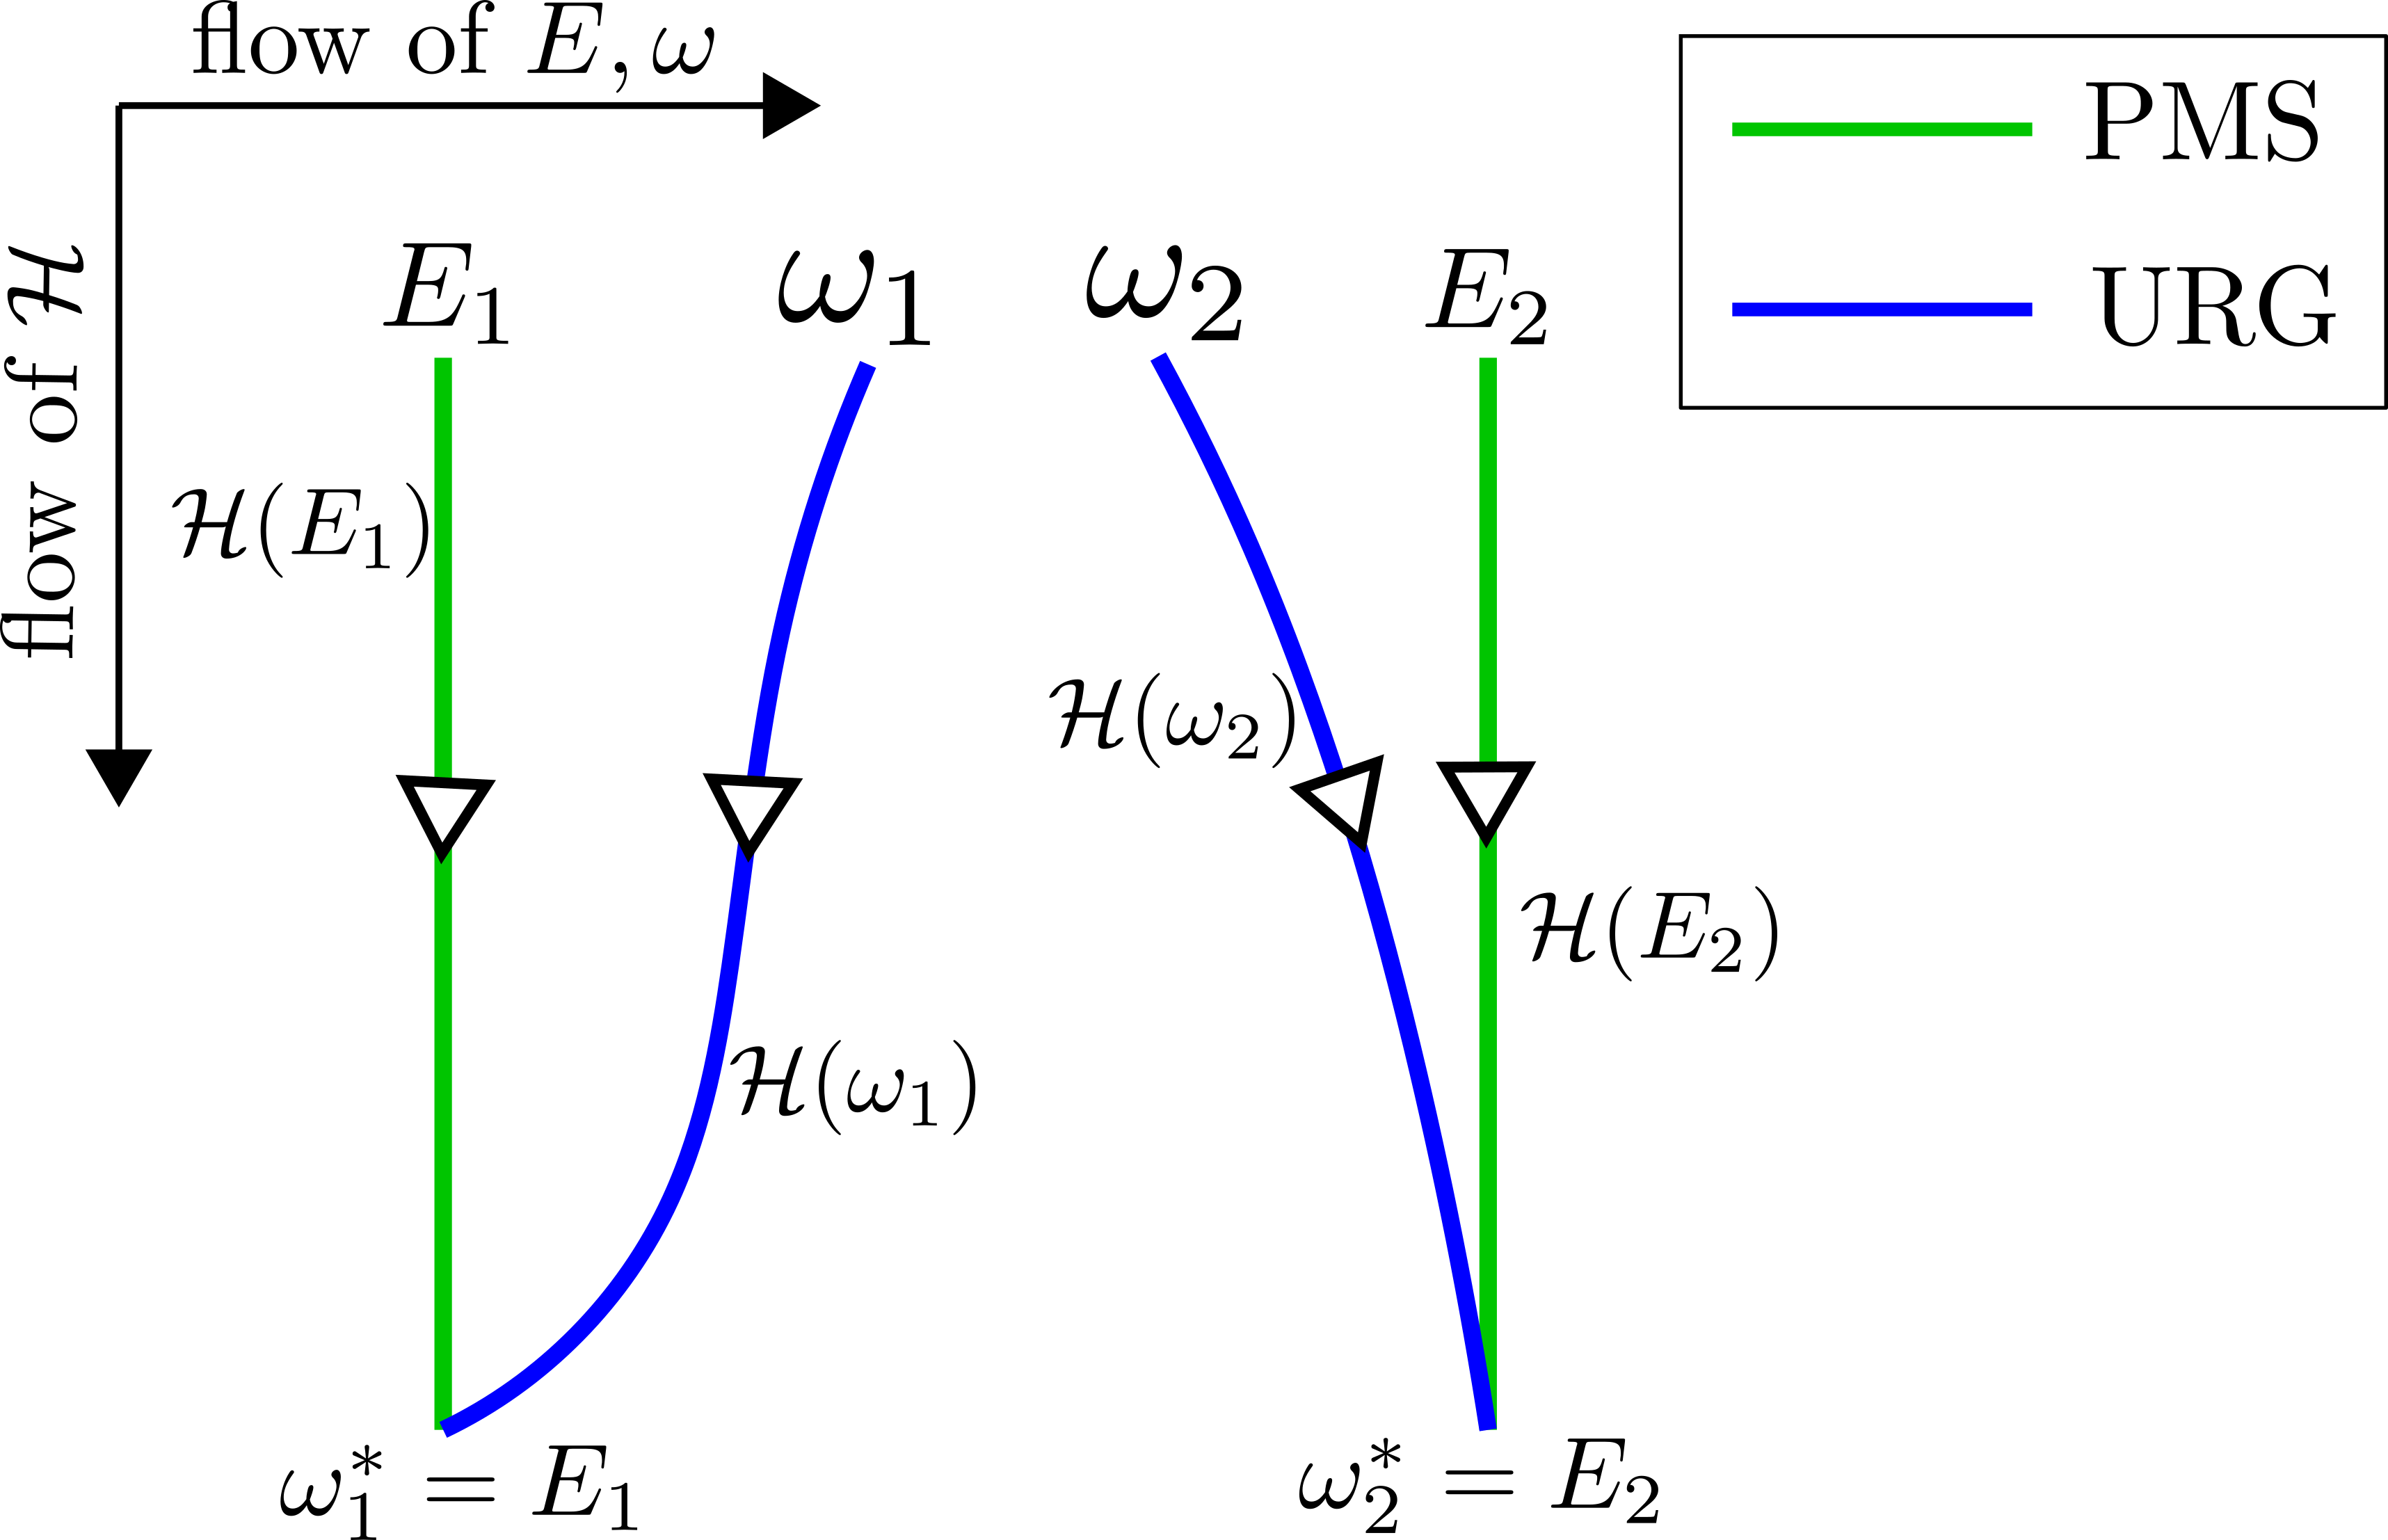
\includegraphics[width=0.6\textwidth]{pms_vs_urg.png}
\caption{Flows of PMS(green) and URG(blue)}
\end{figure}
\subsection{PMS for the single impurity Anderson model}
To demonstrate the implementation, we can look at a specific model. For the SIAM,
\begin{equation}\begin{aligned}
	\mathcal{H} = \sum_{k\sigma}\left(\epsilon_k \tau_{k\sigma} + V c^\dagger_{k\sigma}c_{d\sigma} + \text{h.c.}\right)
\end{aligned}\end{equation}
where \(\tau = \hat n - \frac{1}{2}\). We want to decouple the state \(q\beta\) from the rest of the electrons. We have \({H}_0 = \epsilon_d\hat n_d + U \hat n_{d\uparrow}n_{d\downarrow} + \sum_{k\sigma} \epsilon_k \hat n_{k\sigma}\), \(V_0 = \sum_{k<q,\sigma}c^\dagger_{k\sigma}c_{d\sigma}+\text{h.c.}\), \(V_+ = V c^\dagger_{q\beta}c_{d\beta}\) and \(V_- = V c^\dagger_{d\beta}c_{q\beta}\). The renormalization in particle sector
\begin{equation}\begin{aligned}
	\Delta V_0 &=  c^\dagger_{d\beta}c_{q\beta}\frac{1}{\left(E - V_0\right) - \hat{\mathcal{H}}^d_0}c^\dagger_{q\beta}c_{d\beta}\\
\end{aligned}\end{equation}
The intermediate energy (at the propagator) is
\begin{equation}\begin{aligned}
	\hat{\mathcal{H}}^d_0 = \sum_{k,\sigma}\epsilon_k \tau_{k\sigma} + \epsilon_d \hat n_{d\overline\beta}
\end{aligned}\end{equation}
This is because the \(c_{d\beta}\) at the right of the propagator ensures that we must have \(\hat n_{d\beta}=0\) at the propagator.
\begin{equation}\begin{aligned}
	\Delta V_0 &=  c^\dagger_{d\beta}c_{q\beta}\frac{1}{\left(E - V_0\right) - \sum_{k,\sigma}\epsilon_k \tau_{k\sigma} - \epsilon_d \hat n_{d\overline\beta}}c^\dagger_{q\beta}c_{d\beta}\\
\end{aligned}\end{equation}
Since \(E\) is the exact eigenvalue, we do not have an expression for it. Instead, we approximate \(E - V_0\) by substituting it with the current diagonal part corresponding to the initial state on which this entire term will act. The intial state is characterized by \(\hat n_{q\beta}=0\) and \(\hat n_{d\beta} = 1\), so
\begin{equation}\begin{aligned}
	E - V_0= \sum_{k<q,\sigma}\epsilon_k \tau_{k\sigma} - \frac{1}{2}\epsilon_q + \epsilon_d + \left(\epsilon_d + U\right)\hat n_{d\overline\beta}
\end{aligned}\end{equation}
The \(- \frac{1}{2}\epsilon_q\) comes from substituting \(\hat n_{q\beta}=0\) in \(\epsilon_q \tau_{q\beta}\).

Substituting this in \(\Delta V_0\) gives
\begin{equation}\begin{aligned}
\Delta V_0 &=  c^\dagger_{d\beta}c_{q\beta}\frac{1}{-\frac{1}{2}\epsilon_q -\epsilon_q \tau_{q\beta} + \epsilon_d + U\hat n_{d\overline\beta}}c^\dagger_{q\beta}c_{d\beta}\\
&=  c^\dagger_{d\beta}c_{q\beta}\frac{1}{-\epsilon_q + \epsilon_d + U\hat n_{d\overline\beta}}c^\dagger_{q\beta}c_{d\beta}\\
&=  c^\dagger_{d\beta}c_{q\beta}c^\dagger_{q\beta}c_{d\beta}\frac{1}{-\epsilon_q + \epsilon_d + U\hat n_{d\overline\beta}}\\
&=  -c^\dagger_{d\beta}c_{q\beta}c^\dagger_{q\beta}c_{d\beta}\frac{1}{\epsilon_q - \epsilon_d - U\hat n_{d\overline\beta}}\\
&=  \left(1 - \hat n_{q\beta}\right)\left(\frac{-\hat n_{d\beta}\hat n_{d\overline\beta}}{\epsilon_q - \epsilon_d - U} + \frac{-\hat n_{d\beta}\left(1 - \hat n_{d\overline\beta}\right)}{\epsilon_q - \epsilon_d}\right)\\
\end{aligned}\end{equation}
On the second line, we substituted \(\tau_{q\beta} = \frac{1}{2}\) in the denominator, which is ensured by the \(c^\dagger_{q\beta}\) to the right of the propagator. The first term renormalizes the energy of the doublon state and the second term renormalizes that of the singly-occupied state:
\begin{equation}\begin{aligned}
\Delta E_2 &= \frac{-1}{\epsilon_q - \epsilon_d - U}\\
\Delta E_1 &= \frac{-1}{\epsilon_q - \epsilon_d}
\end{aligned}\end{equation}
The renormalization in the hole sector is
\begin{equation}\begin{aligned}
	\Delta V_0 &=  c^\dagger_{q\beta}c_{d\beta}\frac{1}{\left(E - V_0\right) - \hat {\mathcal{H}}^d_0}c^\dagger_{d\beta}c_{q\beta}\\
		   &=  c^\dagger_{q\beta}c_{d\beta}\frac{1}{\left(E - V_0\right) - \sum_{k,\sigma}\epsilon_k\tau_{k\sigma} - \epsilon_d - \left(\epsilon_d + U\right)\hat n_{d\overline\beta}}c^\dagger_{d\beta}c_{q\beta}
\end{aligned}\end{equation}
This time we substitute
\begin{equation}\begin{aligned}
E - V_0 &= \sum_{k<q,\sigma}\epsilon_k \tau_{k\sigma} + \tau_{q\beta} \epsilon^-_q + \epsilon_d\hat n_{d\overline\beta}\\
&= \sum_{k<q,\sigma}\epsilon_k \tau_{k\sigma} + \frac{1}{2} \epsilon^-_q + \epsilon_d\hat n_{d\overline\beta}\\
\end{aligned}\end{equation}
In the last step we put \(\tau_{q\beta}=\frac{1}{2}\) because the state is occupied in the initial configuratin. Note that since the electron \(q\beta\) was occupied in the intial state, the energy \(\epsilon^-_q\) in this sector must be opposite to that of the particle sector, \(\epsilon_q\). Hence \(\epsilon^-_q = -\epsilon_q\), which gives
\begin{equation}\begin{aligned}
\Delta V_0 & = c^\dagger_{q\beta}c_{d\beta}\frac{1}{-\frac{1}{2} \epsilon_q -\epsilon^-_q\tau_{q\beta} - \epsilon_d - U\hat n_{d\overline\beta}}c^\dagger_{d\beta}c_{q\beta}\\
& = c^\dagger_{q\beta}c_{d\beta}c^\dagger_{d\beta}c_{q\beta}\frac{1}{-\epsilon_q - \epsilon_d - U\hat n_{d\overline\beta}}\\
& = \hat n_{q\beta}\left(\frac{-\left(1 - \hat n_{d\beta}\right)\hat n_{d\overline\beta}}{\epsilon_q + \epsilon_d + U} + \frac{-\left(1 - \hat n_{d\beta}\right)\left(1 - \hat n_{d\overline\beta}\right)}{\epsilon_q + \epsilon_d}\right)\\
\end{aligned}\end{equation}
In the second line, we put \(\epsilon^-_q = -\epsilon_q\) and \(\tau_{q\beta} = -\frac{1}{2}\). The first term renormalizes the singly-occupied state while the second term renormalizes the holon state. Combining with the particle sector results, the total renormalization in all the three impurity states (holon, single and doublon) are
\begin{equation}\begin{aligned}
\Delta E_0 &= -\frac{1}{\epsilon_q + \epsilon_d}\\
\Delta E_1 &= -\frac{1}{\epsilon_q + \epsilon_d + U} - \frac{1}{\epsilon_q - \epsilon_d}\\
\Delta E_2 &= -\frac{1}{\epsilon_q - \epsilon_d - U}\\
\end{aligned}\end{equation}
These results are also obtained in ref.~\cite{hewson}. The complete process is depicted in fig.~\ref{pmsflow}.
\begin{figure}
    \centering
    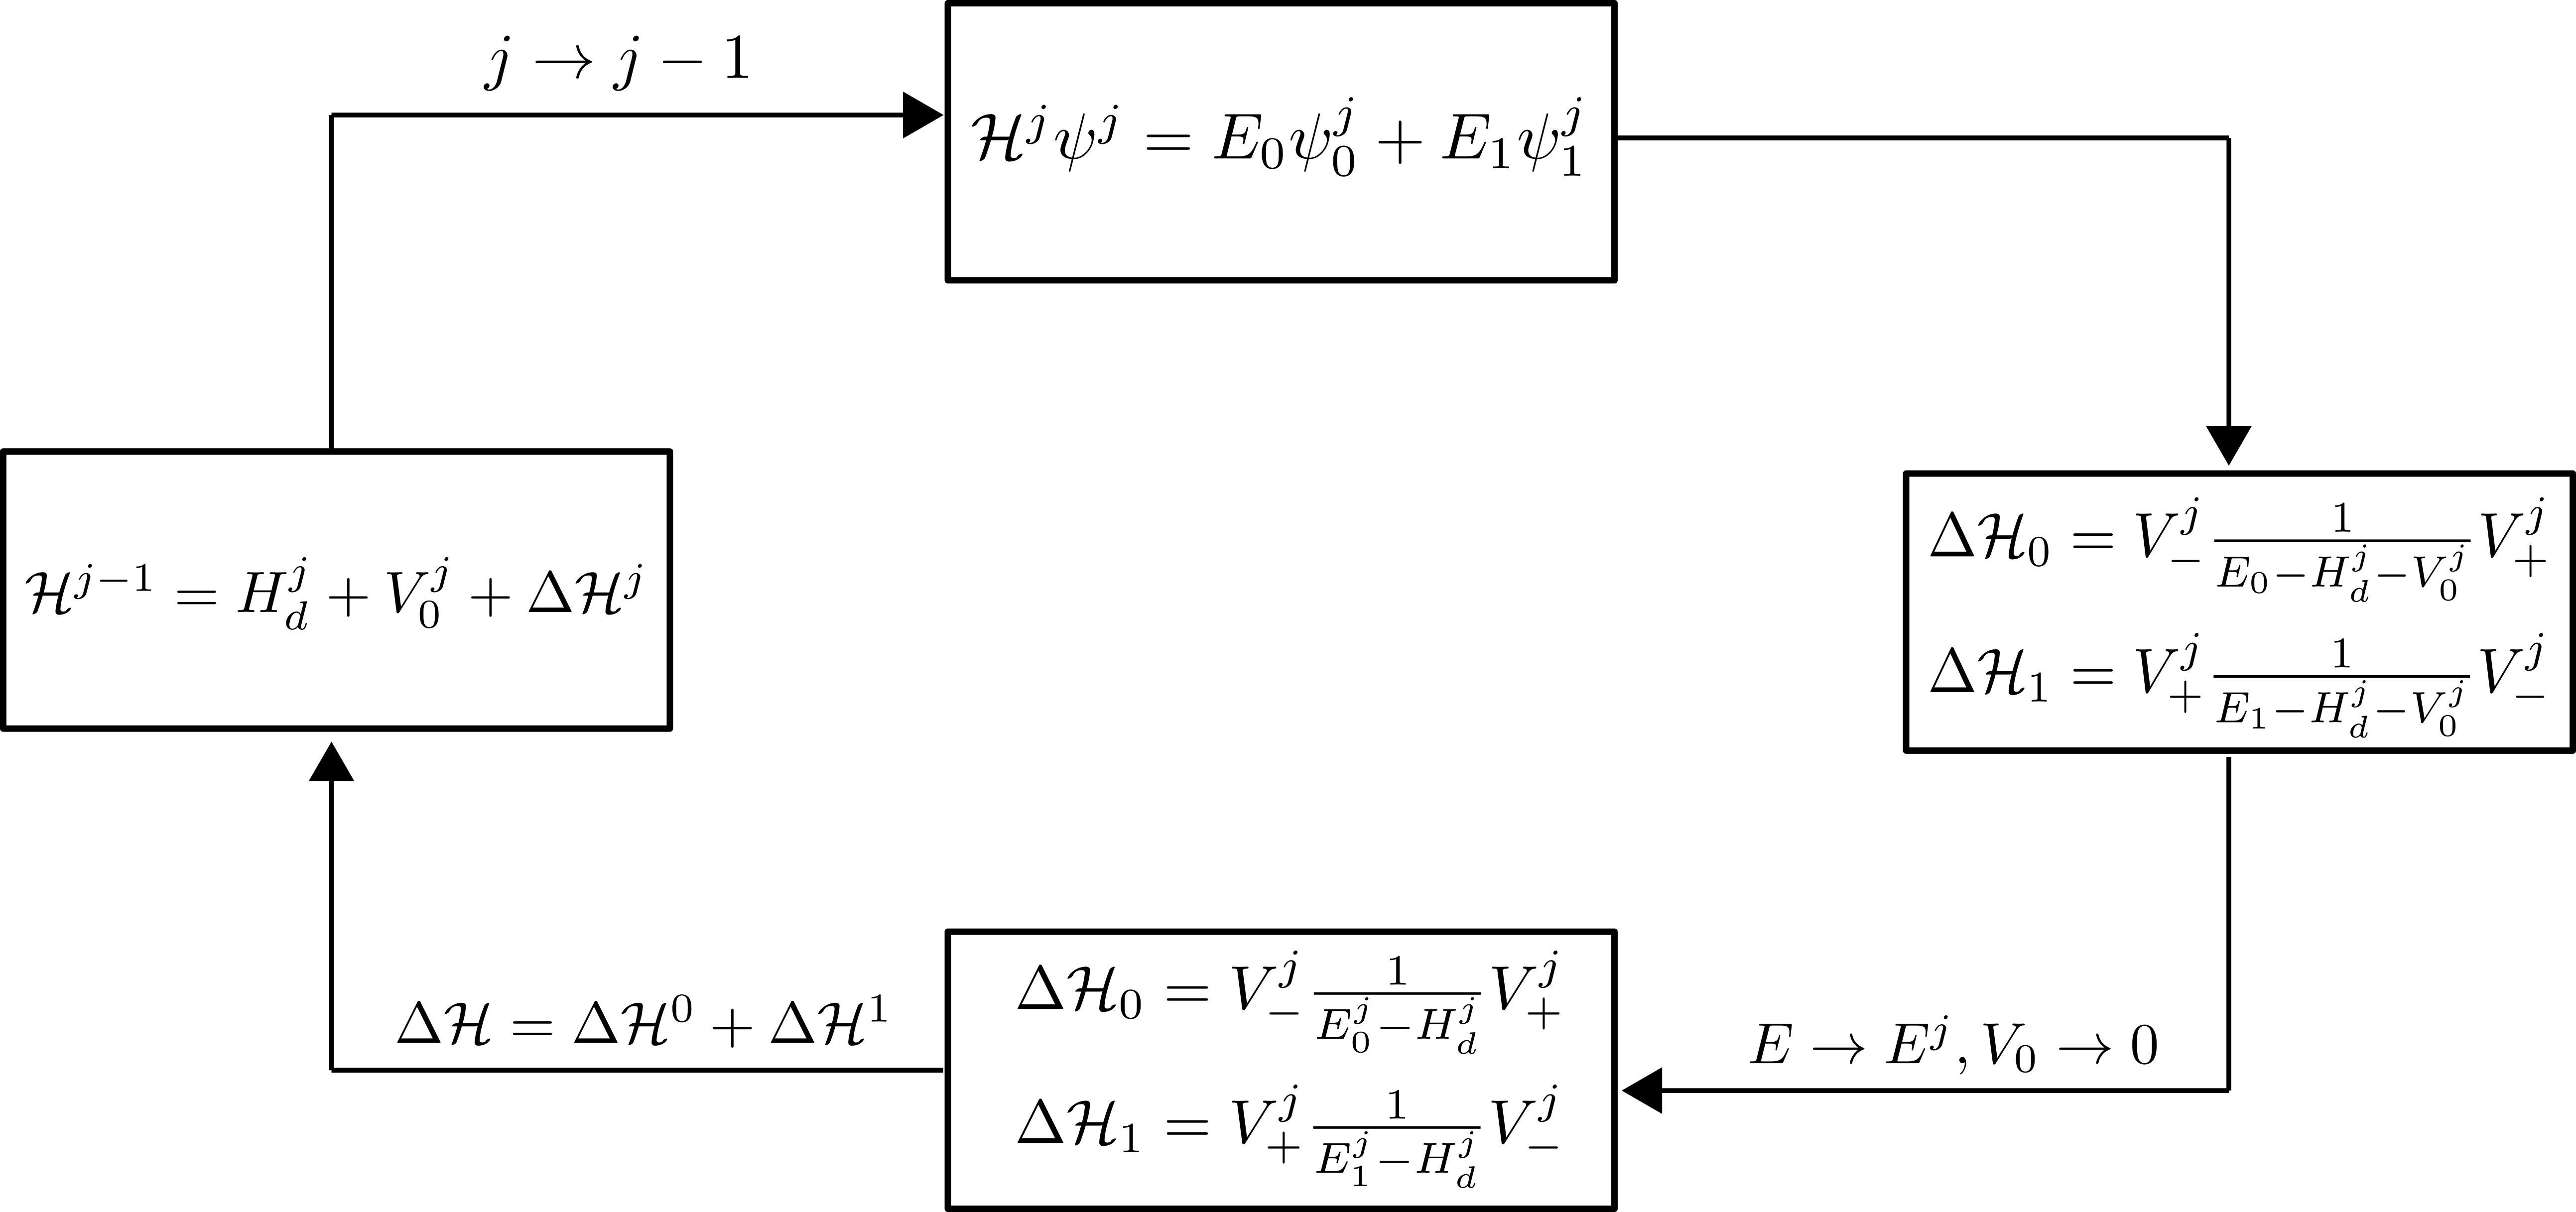
\includegraphics[scale=0.34]{pms-flowchart.png}
    \caption{Flow chart of "Poor Man's" scaling algorithm}
    \label{pmsflow}
\end{figure}

\textbf{Some conclusions}:
\begin{itemize}
\item The \textit{only} difference in the formalism of PMS and URG is that while PMS uses the exact energy eigenvalue \(E\) to parameterise the flow, URG uses a general intermediate decoupled Hamiltonian to do the same. Since the \(E\) is also, technically, an intermediate decoupled Hamiltonian (it is the final Hamiltonian), PMS can be seen as an URG but with a specific choice for the paramter.
\item In practise, PMS replaces \(E-V_0\) with the diagonal part of the initial state at the current step of the RG. We are talking about the energy of the initial state, not the intermediate state. This is because, from eq.~\ref{problem}, \(E\) is the energy of the initial state on which \(V_\pm\) act. 
\item The ideal solution would have been to substitute the exact energy and the total scattering term \(V\), but since we do not know \(E\) and keeping the \(V\) would make the thing untractable, we use our current best guess (renormalised diagonal part). As the RG flows, both \(E_j\) and \(V\) flow, such that at the fixed point, \(V\) becomes zero (scattering terms get removed) and \(E_j\) morphs into the exact \(E\). 
\item In practise, URG replaces the \(\hat \omega\) with a guess for the final energy \(E\). This however ignores the renormalization of \(\hat \omega\). A better approach would be to replace it with \(E_j\), following PMS. That would act like the one-particle renormalization of \(\hat \omega\).
\item PMS usually drops any diagonal component of the scattering from the denominator. For example, in the PMS of the Kondo model by Anderson \cite{Anderson} or that of the anisotropic power law Kondo model by Chenge et.al \cite{tatha}, they do not keep the term \(J_z S_d^z s^z\) in the denominator although it is number(spin) conserving. Such terms are kept in the denominator of the URG though. It must be mentioned however that ref.~\cite{raja} \textit{does} bring a diagonal charge-charge interaction in the denominator in the PMS of the extended Anderson model.
\end{itemize}
\section{Schrieffer-Wolff transformation (SWT)}\label{sc_wl_t}
\subsection{Formalism}
We have a general Hamiltonian
\begin{equation}\begin{aligned}
\mathcal{H} = \mathcal{H}_0 + \mathcal{H}_X
\end{aligned}\end{equation}
\(\mathcal{H}_0\) is diagonal w.r.t a particular degree of freedom. \(V\) is off-diagonal w.r.t that same degree of freedom. Let \(S\) be an \textit{anti-Hermitian} and \textit{off-diagonal} operator. \(U = e^S\) is then a unitary transformation.
\begin{equation}\begin{aligned}
	U \mathcal{H} U^\dagger &= e^S \left(\mathcal{H}_0 + \mathcal{H}_X\right)e^{-S}\\
				&= \left(\cosh\left(S\right) + \sinh\left(S\right)\right)\left(\mathcal{H}_0 + \mathcal{H}_X\right)\left(\cosh\left(S\right) - \sinh\left(S\right)\right)\\
         &= H_1 + H_2
\end{aligned}\end{equation}
where \(H_1\) is diagonal and \(H_2\) is off-diagonal.
\begin{equation}\begin{aligned}
	H_1=\cosh\left(S\right) \mathcal{H}_0 \cosh\left(S\right) - \sinh\left(S\right) \mathcal{H}_0 \sinh\left(S\right) -\cosh\left(S\right) \mathcal{H}_X \sinh\left(S\right)\\
	+\sinh\left(S\right) \mathcal{H}_X \cosh\left(S\right)\\
	H_2 = - \cosh\left(S\right) \mathcal{H}_0 \sinh\left(S\right) + \sinh\left(S\right) \mathcal{H}_0 \cosh\left(S\right) +\cosh\left(S\right) \mathcal{H}_X \cosh\left(S\right)\\
	-\sinh\left(S\right) \mathcal{H}_X \sinh\left(S\right)
\end{aligned}\end{equation}
The decoupling condition is \(H_2=0\).

For small \(S\), we have \(\sinh S \sim S\) and \(\cosh S \sim 1 + \frac{1}{2} S^2\). Therefore, the off-diagonal part, up to second order, is 
\begin{equation}\begin{aligned}
	H_2 = -\mathcal{H}_0 S + S \mathcal{H}_0 + \mathcal{H}_X + O(S^3) = \left[S,\mathcal{H}_0\right] + \mathcal{H}_X
\end{aligned}\end{equation}
The second order decoupling condition is thus
\begin{equation}\begin{aligned}
	\label{dec_cond}
	\left[S,\mathcal{H}_0\right] = -\mathcal{H}_X
\end{aligned}\end{equation}
The effective Hamiltonian is what remains, \(H_1\). That becomes, at second order,
\begin{equation}\begin{aligned}
	H_1 &= \left(1 + \frac{1}{2} S^2\right) \mathcal{H}_0 \left(1 + \frac{1}{2} S^2\right) - S \mathcal{H}_0 S -\left(1 + \frac{1}{2} S^2\right) \mathcal{H}_X S + S \mathcal{H}_X \left(1 + \frac{1}{2} S^2\right)\\
    &= \mathcal{H}_0 + \frac{1}{2} \left\{S^2, \mathcal{H}_0\right\} - S \mathcal{H}_0 S - \mathcal{H}_X S + S \mathcal{H}_X + O(S^3)\\
    &= \mathcal{H}_0 + \frac{1}{2} S\left[S, \mathcal{H}_0\right] - \frac{1}{2} \left[S, \mathcal{H}_0\right]S  + \left[S,\mathcal{H}_X\right] + O(S^3)\\
    &= \mathcal{H}_0 + \frac{1}{2} \left[S,\left[S, \mathcal{H}_0\right]\right] + \left[S,\mathcal{H}_X\right] + O(S^3)\\
    &= \mathcal{H}_0 + \frac{1}{2} \left[S,-\mathcal{H}_X\right] + \left[S,\mathcal{H}_X\right] + O(S^3)\\
    &= \mathcal{H}_0 + \frac{1}{2}\left[S,\mathcal{H}_X\right] + O(S^3)\\
\end{aligned}\end{equation}
Avoiding the perturbative route, we can take \(S = \frac{\pi}{4}\left(\eta^\dagger - \eta\right)\), where \(\eta\) and its conjugate are non-perturbative and Fermionic - they satisfy \(\eta^2 = {\eta^\dagger}^2 = 0\) and \(\left\{\eta,\eta^\dagger\right\}=1\). We can then write
\begin{equation}\begin{aligned}
	e^S &= \exp\left\{\frac{\pi}{4}\left(\eta^\dagger - \eta\right)\right\} \\
	    &= 1 + \left(\eta^\dagger - \eta\right)\frac{\pi}{4} + \frac{1}{2!}\left(\eta^\dagger - \eta\right)^2\left(\frac{\pi}{4}\right)^2 + \frac{1}{3!}\left(\eta^\dagger - \eta\right)^3\left(\frac{\pi}{4}\right)^3 + ...\\
	    &= 1 + \left(\eta^\dagger - \eta\right)\frac{\pi}{4} - \frac{1}{2!}\left(\frac{\pi}{4}\right)^2 - \frac{1}{3!}\left(\eta^\dagger - \eta\right)\left(\frac{\pi}{4}\right)^3 + \frac{1}{4!}\left(\frac{\pi}{4}\right)^4 + ...\\
	    &= \cos \frac{\pi}{4} + \left(\eta^\dagger - \eta\right)\sin\frac{\pi}{4}\\
	    &= \frac{1}{\sqrt 2}\left(1 + \eta^\dagger - \eta\right)
\end{aligned}\end{equation}
There we used
\begin{equation}\begin{aligned}
	\left(\eta^\dagger - \eta\right)^2 = {\eta^\dagger}^2 + \eta^2 - \left\{\eta^\dagger,\eta\right\} = -1 &&\left[\because\eta^2 = {\eta^\dagger}^2=0\right]
\end{aligned}\end{equation}
and hence
\begin{equation}\begin{aligned}
	\left(\eta^\dagger - \eta\right)^3 = -1\left(\eta^\dagger - \eta\right)
\end{aligned}\end{equation}
and so on. This simplification allows us to write
\begin{equation}\begin{aligned}
	\label{cossin}
	\cosh S = \frac{1}{2}\left[e^S + e^{-S}\right] = \frac{1}{2\sqrt 2}\left(1 + \eta^\dagger - \eta + 1 - \eta^\dagger + \eta\right) = \frac{1}{\sqrt 2}
\end{aligned}\end{equation}
and
\begin{equation}\begin{aligned}
	\sinh S = \frac{1}{2}\left[e^S - e^{-S}\right] = \frac{1}{2\sqrt 2}\left(1 + \eta^\dagger - \eta - 1 + \eta^\dagger - \eta\right) = \frac{1}{\sqrt 2}\left(\eta^\dagger - \eta\right)
\end{aligned}\end{equation}
The off-diagonal part now becomes
\begin{equation}\begin{aligned}
	H_2 = \frac{1}{2}\left(\mathcal{H}_X - \eta^\dagger \mathcal{H}_X \eta^\dagger - \eta \mathcal{H}_X \eta + \left[\eta^\dagger - \eta, \mathcal{H}_0\right]\right)
\end{aligned}\end{equation}
The vanishing of this quantity is now the decoupling condition, and is also given in eq 16 of ref.~\cite{anirbanurg1}.

To look for a decoupling condition similar to eq.~\ref{dec_cond}, we can re-express the \(\cosh\) and \(\sinh\) in eq.~\ref{cossin} in terms of \(S\), by substituting \(\eta^\dagger - \eta = \frac{4}{\pi}S\):
\begin{equation}\begin{aligned}
\cosh S = \frac{1}{\sqrt 2},\text{ and } \sinh S = \frac{4}{\sqrt 2 \pi}S
\end{aligned}\end{equation}
That gives
\begin{equation}\begin{aligned}
	H_2 = \frac{1}{2}\left(\frac{4}{\pi}\left[S,\mathcal{H}_0\right] + \mathcal{H}_X - \frac{16}{\pi^2}S \mathcal{H}_X S\right)
\end{aligned}\end{equation}
The decoupling condition becomes
\begin{equation}\begin{aligned}
	\left[S,\mathcal{H}_0\right] = -\frac{\pi}{4}\mathcal{H}_X + \frac{4}{\pi}S \mathcal{H}_X S
\end{aligned}\end{equation}
This can be compared to the second order condition: \(\left[S,\mathcal{H}_0\right] = -\mathcal{H}_X\). We  can also write the effective Hamiltonian for this non-perturbative case.
\begin{equation}\begin{aligned}
	U\mathcal{H} U^\dagger = H_1 = \frac{1}{2} \mathcal{H}_0 - \frac{4}{\pi^2}S\mathcal{H}_0 S  + \frac{2}{\pi}\left[S,\mathcal{H}_X\right]
\end{aligned}\end{equation}
The differences between the perturbative and non-perturbative ways are summarized in table \ref{comparison}.
\begin{table}
% \def\tabcolsep=10pt
\centering
\begin{tabular}{|c|c|c|}
    \hline
        &renormalization&decoupling condition\\
    \hline
	SWT&\(\frac{1}{2} \left[S,\mathcal{H}_X\right]\)&\(\left[S,\mathcal{H}_0\right] = -\mathcal{H}_X\)\\
	URG&\(\frac{2}{\pi}\left[S,\mathcal{H}_X\right]\)&\(\left[S,\mathcal{H}_0\right] = -\frac{\pi}{4}\mathcal{H}_X + \frac{4}{\pi}S \mathcal{H}_X S\)\\
    \hline
\end{tabular}
    \caption{Comparison of perturbative and non-perturbative canonical transformations}
    \label{comparison}
\end{table}
There appear to be two differences between these decoupling conditions: (a)  a pre-factor of \(\frac{\pi}{4}\) for the first term on the right hand side, and (b) the altogether new second term on the right hand side. Both are outcomes of the non-perturbative nature of URG. This offers evidence that the physics captured by the effective Hamiltonian (and its associated low-energy many-particle Hilbert space) obtained from URG lies well beyond that obtained from SWT. Further, it shows that the SWT can only be justified as an expansion in a small parameter (say, $\frac{1}{U}$) in the Anderson impurity problem), followed by a truncation of the BCH expansion and a projection onto a particular low-energy subspace. The truncation and projection are adopted simultaneously, and appear to impose the limit of \(U = \infty\) by hand. The URG flow never attains such a limit, thus suggesting that there exists a lot of interesting physics that could potentially be lost in the SWT procedure. Further, the projection finally applied within SWT means that we can never recover what is thrown away. This is again not the case with URG.
\subsection{Obtaining renormalization via Schrieffer-Wolff transformation - comparison with "poor man's scaling" and URG}
Similar to the situation in Poor Man's scaling, one can visualize two set of states and let \(\mathcal{H}_X = V_+ + V_-\) be the scattering that connects them and hence the one we want to kill. Let \(S\) be of the form 
\begin{equation}\begin{aligned}
	S = \sum_{ij}\left[s\ket{\phi_1^i}\bra{\phi_0^j} - s^\dagger\ket{\phi_0^j}\bra{\phi_1^i}\right]
\end{aligned}\end{equation}
This form is of course chosen to make \(S\) anti-Hermitian and off-diagonal. The part \(s\) can be determined from the decoupling condition:
\begin{equation}\begin{aligned}
	-\mathcal{H}_X = \left[S, H_0\right] = S H_0 - H_0 S
\end{aligned}\end{equation}
Multiplying with \(\bra{\phi_0^a}\) and \(\ket{\phi_1^b}\) from the left and right respectively gives
\begin{equation}\begin{aligned}
-\bra{\phi_0^a}V + V^\dagger\ket{\phi_1^b} &= \bra{\phi_0^a}S H_0 - H_0 S\ket{\phi_1^b}\\
\end{aligned}\end{equation}
Since \(V^\dagger\) acts on \(\ket{0}\), it will not affect the LHS. Also, \(\bra{\phi_0^a}V\ket{\phi_1^b} = V_{ab}\). If we now consider only the diagonal part of \(H_0\), we can write \(H_0 (\ket{\phi_0^a},\ket{\phi_1^b}) = (E_{0,a}\ket{\phi_0^a},E_{1,b}\ket{\phi_1^b}))\). We then get
\begin{equation}\begin{aligned}
	-V_{ab} &= \bra{\phi_0^a}\sum_i\left[S\ket{\phi_1^i}\bra{\phi_1^i} H_0 - H_0 \ket{\phi_0^i}\bra{\phi_0^i}S\right]\ket{\phi_1^b}\\
		&= \sum_i\left[S_{ai}E_1^i \delta_{bi} - E^i_0 \delta_{ai}S_{ib}\right]\\
    &= S_{ab}E_1^b  - E^a_0 S_{ab}\\
\implies S_{ab} &= \frac{V_{ab}}{E_0^a - E_1^b}
\end{aligned}\end{equation}
where we defined \(\bra{\phi_0^x}S\ket{\phi_1^y} = S_{xy}\). The total generator is
\begin{equation}\begin{aligned}
	\label{swtgen}
	S &= \sum_{ij}\left[S_{ij}\ket{\phi_0^i}\bra{\phi_1^j} - S_{ij}^\dagger\ket{\phi_1^j}\bra{\phi_0^i}\right]\\
	  &= \sum_{ij}\frac{1}{E_0^i - E_1^j}\left[V_{ij}\ket{\phi_0^i}\bra{\phi_1^j} - V^\dagger_{ij}\ket{\phi_1^j}\bra{\phi_0^i}\right]\\
\end{aligned}\end{equation}
The renormalization is thus
\begin{equation}\begin{aligned}
	\Delta \mathcal{H} &= \frac{1}{2} \left[S,\mathcal{H}_X\right]\\
			   &= \frac{1}{2} \sum_{ij,kl}\left[\frac{1}{E_0^i - E_1^j}\left(V_{ij}\ket{\phi_0^i}\bra{\phi_1^j} - V^\dagger_{ij}\ket{\phi_1^j}\bra{\phi_0^i}\right), V_{kl} \ket{\phi_0^k}\bra{\phi_1^l}+ V^\dagger_{kl} \ket{\phi_1^l}\bra{\phi_0^k}\right]\\
                  &= \frac{1}{2} \sum_{ij,kl}\left[\frac{1}{E_0^i - E_1^j}\left(V_{ij}V^\dagger_{kl}\ket{\phi_0^i}\bra{\phi_0^k}\delta_{jl} - V^\dagger_{ij}V_{kl}\ket{\phi_1^j}\bra{\phi_1^l}\delta_{ik}\right.\right.\\
                  &\quad\left.\left.- V^\dagger_{kl}V_{ij}\ket{\phi_1^l}\bra{\phi_1^j}\delta_{ki} + V_{kl}V^\dagger_{ij}\ket{\phi_0^k}\bra{\phi_0^i}\delta_{lj}\right)\right]\\
                  &= \frac{1}{2} \sum_{ijk}\left[\frac{1}{E_0^i - E_1^j}\left(V_{ij}V^\dagger_{kj}\ket{\phi_0^i}\bra{\phi_0^k} - V^\dagger_{ij}V_{ik}\ket{\phi_1^j}\bra{\phi_1^k}- V^\dagger_{ik}V_{ij}\ket{\phi_1^k}\bra{\phi_1^j} + V_{kj}V^\dagger_{ij}\ket{\phi_0^k}\bra{\phi_0^i}\right)\right]\\
		  &= \frac{1}{2} \sum_{ijk}\left[\left(\frac{1}{E_0^i - E_1^j} + \frac{1}{E_0^k - E_1^j}\right)V_{ij}V^\dagger_{kj}\ket{\phi_0^i}\bra{\phi_0^k} - \left(\frac{1}{E_0^i - E_1^j} + \frac{1}{E_0^i - E_1^k}\right)V^\dagger_{ij}V_{ik}\ket{\phi_1^j}\bra{\phi_1^k}\right]\\
\end{aligned}\end{equation}
This is the same as the PMS result eq.~\ref{pmsren}. It is easy to see that since this transformation is unitary, it has zero trace so as to preserve the trace of the Hamiltonian:
\begin{equation}\begin{aligned}
	\text{Tr}\left[\mathcal{H}\right] &= \sum_{l}\left(\bra{\phi_0^l} + \bra{\phi_1^l}\right)\Delta \mathcal{H}\left(\ket{\phi_0^l} + \ket{\phi_1^l}\right)\\
		&= \frac{1}{2} \sum_{jl}\frac{2}{E_0^l - E_1^j}V_{lj}V^\dagger_{lj} - \frac{1}{2} \sum_{ji}\frac{2}{E_0^i - E_1^l}V^\dagger_{il}V_{il}\\
		&= 0
\end{aligned}\end{equation}

We can also make a comparison to the renormalization obtained from URG.
\begin{equation}\begin{aligned}
	\Delta \mathcal{H} &= \frac{1}{2}\left[\eta^\dagger - \eta,\mathcal{H}\right]
\end{aligned}\end{equation}
where 
\begin{equation}\begin{aligned}
\eta &= \frac{1}{\omega - \mathcal{H}^d}\sum_{ij}V_{ij}\ket{\phi_0^i}\bra{\phi_1^j} = \sum_{ij}\frac{1}{\omega_1^j - E_0^i}V_{ij}\ket{\phi_0^i}\bra{\phi_1^j}\\
\implies \eta^\dagger &= \sum_{ij}\frac{1}{\omega_1^j - E_0^i}V^\dagger_{ij}\ket{\phi_1^j}\bra{\phi_0^i}\\
\implies \eta^\dagger - \eta &= \sum_{ij}\frac{1}{\omega_1^j - E_0^i}\left(V^\dagger_{ij}\ket{\phi_1^j}\bra{\phi_0^i} - V_{ij}\ket{\phi_0^i}\bra{\phi_1^j}\right)\\
\end{aligned}\end{equation}
This can be thought of as the generator for the unitary transformations of URG. Comparing with the generator \(S\) of eq.~\ref{swtgen}, the prescription to go from URG to SWT is to replace \(\omega_1^j \to E_1^j\). Doing a similar calculation gives
\begin{equation}\begin{aligned}
	\Delta \mathcal{H}_{URG} = \frac{1}{2} \sum_{ijk}\left[\left(\frac{1}{E_0^i - \omega_1^j} + \frac{1}{E_0^k - \omega_1^j}\right)V_{ij}V^\dagger_{kj}\ket{\phi_0^i}\bra{\phi_0^k}\right.\\
	- \left.\left(\frac{1}{E_0^i - \omega_1^j} + \frac{1}{E_0^i - \omega_1^k}\right)V^\dagger_{ij}V_{ik}\ket{\phi_1^j}\bra{\phi_1^k}\right]\\
\end{aligned}\end{equation}

\section{A comparison of URG, SWT and PMS on the Anderson model}
The SWT for the single-impurity Anderson model is briefly sketched below. In order to decouple a state \(q\beta\) from the SIAM (\(\epsilon_q > 0\)) , we take an ansatz \(S = (A + B\hat n_{d\overline\beta})(c^\dagger_{q\beta}c_{d\beta} - \text{h.c.})\). Plugging this into the decoupling condition gives
\begin{equation}\begin{aligned}
	-\epsilon_q\left(A + B\hat n_{d\overline\beta}\right) + \epsilon_d\left(A + B\hat n_{d\overline\beta}\right) + U\left(A + B\right)\hat n_{d\overline\beta} = -V
\end{aligned}\end{equation}
which gives
\begin{equation}\begin{aligned}
	S = V\left[\frac{1 - \hat n_{d\overline\beta}}{\epsilon_q - \epsilon_d} + \frac{\hat n_{d\overline\beta}}{\epsilon_q - \epsilon_d - U}\right] (c^\dagger_{q\beta}c_{d\beta} - \text{h.c.})
\end{aligned}\end{equation}
The remaining diagonal part constitutes the effective Hamiltonian.
\begin{equation}\begin{aligned}
	U\mathcal{H} U^\dagger = H_1 &= \mathcal{H}_0 + \frac{1}{2} \left\{\mathcal{H}_0, S^2\right\} - S \mathcal{H}_0 S + \left[S,\mathcal{H}_X\right]\\
				     &=\mathcal{H}_0 + \frac{1}{2} \left[\left[\mathcal{H}_0, S\right],S\right] + \left[S,\mathcal{H}_X\right]\\
				     &=\mathcal{H}_0 + \frac{1}{2} \left[\mathcal{H}_X,S\right] + \left[S,\mathcal{H}_X\right]\\
				     &=\mathcal{H}_0 + \frac{1}{2} \left[S,\mathcal{H}_X\right]
\end{aligned}\end{equation}
For the SIAM (and noting that we are decoupling \(q\beta\)), the two parts are
\begin{equation}\begin{aligned}
	\mathcal{H}_0 &= \sum_{k\sigma}\epsilon_k \hat n_{k\sigma} + \epsilon_d \hat n_d + U\hat n_{d\uparrow}\hat n_{d\downarrow} + \sum_{k\sigma \neq q\beta}\left(c^\dagger_{k\sigma}c_{d\sigma} + \text{h.c.}\right)\\
\mathcal{H}_X &= c^\dagger_{q\beta}c_{d\beta} + \text{h.c.} 
\end{aligned}\end{equation}
The renormalization in the effective Hamiltonian from decoupling a high energy particle state is thus
\begin{equation}\begin{aligned}
	\frac{1}{2} \left[S,\mathcal{H}_X\right]\bigg\vert_{\hat n_{q\beta}=0} &= |V|^2\left[\frac{1 - \hat n_{d\overline\beta}}{\epsilon_q - \epsilon_d} + \frac{\hat n_{d\overline\beta}}{\epsilon_q - \epsilon_d - U}\right]\left[\hat n_{q\beta}\left(1 - \hat n_{d\beta}\right) - \hat n_{d\beta}\left(1 - \hat n_{q\beta}\right)\right]\bigg\vert_{\hat n_{q\beta}=0}\\
									       &=-\hat n_{d\beta}|V|^2\left[\frac{1 - \hat n_{d\overline\beta}}{\epsilon_q - \epsilon_d} + \frac{\hat n_{d\overline\beta}}{\epsilon_q - \epsilon_d - U}\right]
\end{aligned}\end{equation}
In the last step, we put \(\hat n_{q\beta}=0\) because previously we assumed \(\epsilon_q>0\) and high energy virtual excitations above the Fermi surface must necessarily be vacant in the initial state (at \(T=0\)). We can obtain the renormalization from decoupling a high energy \textit{hole} state directly from this expression, just by choosing \(\hat n_{q\beta}=1\) and setting \(\epsilon_q \to -\epsilon_q\).
\begin{equation}\begin{aligned}
	\frac{1}{2} \left[S,\mathcal{H}_X\right]\bigg\vert_{\hat n_{q\beta}=1} &=-\left(1 - \hat n_{d\beta}\right)|V|^2\left[\frac{1 - \hat n_{d\overline\beta}}{\epsilon_q + \epsilon_d} + \frac{\hat n_{d\overline\beta}}{\epsilon_q + \epsilon_d + U}\right]
\end{aligned}\end{equation}
These two results - the renormalization in the particle and hole sectors - is identical to the result (see \cite{hewson}) obtained from PMS of the SIAM. The renormalizations in the various energy levels of the impurity can be read off now, after summing over all states in the interval we are decoupling.
\begin{equation}\begin{aligned}
\Delta E_2 &= -2\sum_{q}\frac{|V_q|^2}{\epsilon_q - \epsilon_d - U}\\
\Delta E_1 &= -\sum_{q}\frac{|V_q|^2}{\epsilon_q - \epsilon_d} - \sum_{q}\frac{|V_q|^2}{\epsilon_q + \epsilon_d + U}\\
\Delta E_0 &= -2\sum_{q}\frac{|V_q|^2}{\epsilon_q + \epsilon_d}\\
\end{aligned}\end{equation}
This can be compared with the URG result, eq.~\ref{urg-siam},
\begin{equation}\begin{aligned}
\Delta E_2 &= 2\sum_{q}\frac{|V_q|^2}{\omega - \frac{1}{2}\epsilon_q + \epsilon_d + U}\\
\Delta E_1 &= \sum_{q}\frac{|V_q|^2}{\omega - \frac{1}{2}\epsilon_q - \epsilon_d - U} + \sum_{q}\frac{|V_q|^2}{\omega - \frac{1}{2}\epsilon_q + \epsilon_d}\\
\Delta E_0 &= 2\sum_{q}\frac{|V_q|^2}{\omega - \frac{1}{2}\epsilon_q - \epsilon_d}\\
\end{aligned}\end{equation}
We can transform the URG result to the SWT result if we ignore the effect of the quantum fluctuations in \(\omega\) (arising from the presence of the off-diagonal term \(\mathcal{H}^i\)) and replace it with the renormalised diagonal value of \(-\frac{1}{2}\epsilon_q\). This means that SWT tracks the effect of the off-diagonal terms only in the numerator. Of course, all this assumes we are doing an iterative SWT instead of a one-shot SWT; the latter is the conventional way. A second difference is that URG has a Green's function like structure in the renormalization such that a fixed point is reached when the diagonal part \(\mathcal{H}^d\) matches one of the eigenvalues of \(\omega\) (see \ref{match}). SWT does not have such a fixed point structure.

Another point to note is that decoupling a single electron does not generate all the charge-charge or spin-spin interactions that come out when one performs a one-shot SWT. This implies that such terms are a result of decoupling the non-local interactions of the impurity (it is talking to all the mobile electrons), and cannot be generated when we remove just the local interactions of the mobile electrons. Instead, if one performs a URG in which we non-perturbatively kill the 2-point vertices in the SIAM, such 4-point vertices are generated. This is shown in the next subsection.
\section{Deriving the Kondo model from the Anderson model via a one-shot URG}\label{SWT from URG}
Here we will show how we can obtain the spin-spin interaction of the Kondo model by performing a one-shot URG on the SIAM. This should justify that the action of performing an SWT is analogous to decoupling the whole band via URG. 
There are three departures from the conventional way of doing URG (or PMS).
\begin{itemize}
    \item We will be severing the connections of the impurity with all the mobile electrons in one-shot, and not iteratively.
    \item We will have to trivialize the quantum fluctuation operator \(\hat \omega\) by replacing it with the diagonal part of the initial state energy.
\end{itemize}
Since we are decoupling the whole band, the off-diagonal part that we want to remove is
\begin{equation}\begin{aligned}
	\mathcal{H}^I = \sum_{k\sigma}\left[V_k c^\dagger_{k\sigma}c_{d\sigma}+\text{h.c.}\right]
\end{aligned}\end{equation}
The diagonal part is the rest of the Hamiltonian.
\begin{equation}\begin{aligned}
\mathcal{H}^d &= \sum_{k\sigma}\epsilon_k\hat n_{k\sigma} + \epsilon_d\hat n_d + U\hat n_{d\uparrow}\hat n_{d\downarrow}\\
&= \sum_{k\sigma}\epsilon_k\tau_{k\sigma} + \epsilon_d\hat n_d + U\hat n_{d\uparrow}\hat n_{d\downarrow}\\
\end{aligned}\end{equation}
Following eq.~\ref{renurg}, the renormalization is
\begin{equation}\begin{aligned}
	\Delta \mathcal{H} = \frac{1}{2}\left[\eta^\dagger - \eta, \mathcal{H}_X\right]
\end{aligned}\end{equation}
The transition operator \(\eta\) is
\begin{equation}\begin{aligned}
	\label{swturg}
\eta &= \frac{1}{\omega - \mathcal{H}^d}\sum_{k\sigma}V^*_k c^\dagger_{d\sigma}c_{k\sigma}\\
     &= \sum_{k\sigma}\frac{1}{\omega + \frac{1}{2}\epsilon_k - \epsilon_d - \left(\epsilon_d + U\right)\hat n_{d\overline\sigma}}V^*_k c^\dagger_{d\sigma}c_{k\sigma}\\
     &= \sum_{k\sigma}\left[\frac{\hat n_{d\overline\sigma}}{\omega_1 + \frac{1}{2}\epsilon_k - 2\epsilon_d - U} + \frac{1 - \hat n_{d\overline\sigma}}{\omega_0 + \frac{1}{2}\epsilon_k - \epsilon_d}\right]V^*_k c^\dagger_{d\sigma}c_{k\sigma}\\
     &= \sum_{k\sigma}\left[\frac{\hat n_{d\overline\sigma}}{E_k^1} + \frac{1 - \hat n_{d\overline\sigma}}{E_k^0}\right]V^*_k c^\dagger_{d\sigma}c_{k\sigma}\\
\end{aligned}\end{equation}
where \(E_k^1 = \omega_1 + \frac{1}{2}\epsilon_k - 2\epsilon_d - U\) and \(E_k^0 = \omega_0 + \frac{1}{2}\epsilon_k - \epsilon_d\). The total generator is therefore
\begin{equation}\begin{aligned}
	\eta^\dagger - \eta = \sum_{k\sigma}\left[\frac{\hat n_{d\overline\sigma}}{E_k^1} + \frac{1 - \hat n_{d\overline\sigma}}{E_k^0}\right] \left(V_k c^\dagger_{k\sigma}c_{d\sigma} - V^*_k c^\dagger_{d\sigma}c_{k\sigma}\right)
\end{aligned}\end{equation}
The renormalization is
\begin{equation}\begin{aligned}
	\Delta \mathcal{H}(\omega_1,\omega_0) = \frac{1}{2}\sum_{kq\sigma\alpha}\left[\left(\frac{\hat n_{d\overline\sigma}}{E_k^1} + \frac{1 - \hat n_{d\overline\sigma}}{E_k^0}\right)\left(V_k c^\dagger_{k\sigma}c_{d\sigma} - V^*_k c^\dagger_{d\sigma}c_{k\sigma}\right),V_q c^\dagger_{q\alpha}c_{d\alpha} + V_q^* c^\dagger_{d\alpha}c_{q\alpha}\right]
\end{aligned}\end{equation}
The summation has two parts, \(\Delta_{1,2}\) - one where \(\sigma=\alpha\) and another where \(\sigma=\overline\alpha\). The first part \(\Delta_1\) gives
\begin{equation}\begin{aligned}
	\Delta_1 &=\frac{1}{2}\sum_{kq\sigma=\alpha}\left[\left(\frac{\hat n_{d\overline\sigma}}{E_k^1} + \frac{1 - \hat n_{d\overline\sigma}}{E_k^0}\right)\left(V_k c^\dagger_{k\sigma}c_{d\sigma} - V^*_k c^\dagger_{d\sigma}c_{k\sigma}\right),V_q c^\dagger_{q\sigma}c_{d\sigma} + V_q^* c^\dagger_{d\sigma}c_{q\sigma}\right]\\
		 &=\frac{1}{2}\sum_{kq\sigma}\left(\frac{\hat n_{d\overline\sigma}}{E_k^1} + \frac{1 - \hat n_{d\overline\sigma}}{E_k^0}\right)\left[V_k c^\dagger_{k\sigma}c_{d\sigma} - V^*_k c^\dagger_{d\sigma}c_{k\sigma},V_q c^\dagger_{q\sigma}c_{d\sigma} + V_q^* c^\dagger_{d\sigma}c_{q\sigma}\right]\\
		 &=\frac{1}{2}\sum_{kq\sigma}\left(\frac{\hat n_{d\overline\sigma}}{E_k^1} + \frac{1 - \hat n_{d\overline\sigma}}{E_k^0}\right)\left\{V_k V_q^*\left[c^\dagger_{k\sigma}c_{d\sigma}, V_q^* c^\dagger_{d\sigma}c_{q\sigma}\right] - V^*_k V_q \left[c^\dagger_{d\sigma}c_{k\sigma},c^\dagger_{q\sigma}c_{d\sigma}\right]\right\}\\
		 &=\frac{1}{2}\sum_{kq\sigma}\left(\frac{\hat n_{d\overline\sigma}}{E_k^1} + \frac{1 - \hat n_{d\overline\sigma}}{E_k^0}\right)\left\{V_k V_q^*\left[c^\dagger_{k\sigma}c_{d\sigma}, V_q^* c^\dagger_{d\sigma}c_{q\sigma}\right] + V^*_k V_q \left[c^\dagger_{q\sigma}c_{d\sigma},c^\dagger_{d\sigma}c_{k\sigma}\right]\right\}\\
		 &=\frac{1}{2}\sum_{kq\sigma}\left[\hat n_{d\overline\sigma}\left(\frac{1}{E_k^1} + \frac{1}{E_q^1}\right) + \left(1 - \hat n_{d\overline\sigma}\right)\left(\frac{1}{E_k^0} + \frac{1}{E_q^0}\right)\right]V_k V_q^*\left[c^\dagger_{k\sigma}c_{d\sigma}, c^\dagger_{d\sigma}c_{q\sigma}\right]\\
		 &=\sum_{kq\sigma}\left[\frac{1}{2} V_k V_q^*\left(\frac{1}{E_k^0} + \frac{1}{E_q^0}\right) + \hat n_{d\overline\sigma}\frac{1}{2} V_k V_q^*\left(\frac{1}{E_k^1} + \frac{1}{E_q^1} - \frac{1}{E_k^0} - \frac{1}{E_q^0}\right)\right] \left(c^\dagger_{k\sigma}c_{q\sigma} - c^\dagger_{d\sigma}c_{d\sigma}\delta_{kq}\right)\\
\end{aligned}\end{equation}
We can now define two new energy scales:
\begin{equation}\begin{aligned}
	W_{kq} = \frac{1}{2} V_k V_q^*\left(\frac{1}{E_k^0} + \frac{1}{E_q^0}\right),&&&& J_{kq} = \frac{1}{2} V_k V_q^*\left(\frac{1}{E_k^1} + \frac{1}{E_q^1} - \frac{1}{E_k^0} - \frac{1}{E_q^0}\right)
\end{aligned}\end{equation}
The renormalization \(\Delta_1\) becomes
\begin{equation}\begin{aligned}
	\Delta_1 &=\sum_{kq\sigma}\left[W_{kq} + \hat n_{d\overline\sigma}J_{kq}\right] \left(c^\dagger_{k\sigma}c_{q\sigma} - c^\dagger_{d\sigma}c_{d\sigma}\delta_{kq}\right)\\
		 &=\sum_{kq\sigma}\left[W_{kq} + \hat n_{d\overline\sigma}J_{kq}\right]c^\dagger_{k\sigma}c_{q\sigma} - \sum_{k\sigma}\left[W_{kk} + \hat n_{d\overline\sigma}J_{kk}\right]\hat n_{d\sigma}\\
		 &=\sum_{kq\sigma}\left[W_{kq} + \frac{1}{2} \hat n_d J_{kq}\right]c^\dagger_{k\sigma}c_{q\sigma} - \sum_{kq\sigma}\sigma J_{kq} S_d^z c^\dagger_{k\sigma}c_{q\sigma}- \sum_{k\sigma}\left[W_{kk} + \hat n_{d\overline\sigma}J_{kk}\right]\hat n_{d\sigma}
\end{aligned}\end{equation}
There we exchanged \(\hat n_{d\overline\sigma}\) for \(S_d^z\) and \(\hat n_d\), in the first term, by using the definitions \(\hat n_{d\sigma} + \hat n_{d\overline\sigma} = \hat n_{d\sigma}\) and \(\hat n_{d\sigma} - \hat n_{d\overline\sigma} = 2\sigma S_d^z\).

The second term in the summation comes from the choice \(\sigma = \overline\alpha\).
\begin{equation}\begin{aligned}
	\Delta_2 &= \frac{1}{2}\sum_{kq\overline\sigma=\alpha}\left[\left(\frac{\hat n_{d\overline\sigma}}{E_k^1} + \frac{1 - \hat n_{d\overline\sigma}}{E_k^0}\right)\left(V_k c^\dagger_{k\sigma}c_{d\sigma} - V^*_k c^\dagger_{d\sigma}c_{k\sigma}\right),V_q c^\dagger_{q\overline\sigma}c_{d\overline\sigma} + V_q^* c^\dagger_{d\overline\sigma}c_{q\overline\sigma}\right]\\
		 &= \frac{1}{2}\sum_{kq\sigma}\left(V_k c^\dagger_{k\sigma}c_{d\sigma} - V^*_k c^\dagger_{d\sigma}c_{k\sigma}\right)\left[\frac{\hat n_{d\overline\sigma}}{E_k^1} + \frac{1 - \hat n_{d\overline\sigma}}{E_k^0},V_q c^\dagger_{q\overline\sigma}c_{d\overline\sigma} + V_q^* c^\dagger_{d\overline\sigma}c_{q\overline\sigma}\right]\\
		 &= \frac{1}{2}\sum_{kq\sigma}\left(V_k c^\dagger_{k\sigma}c_{d\sigma} - V^*_k c^\dagger_{d\sigma}c_{k\sigma}\right)\left(V_q^*c^\dagger_{d\overline\sigma}c_{q\overline\sigma} - V_q c^\dagger_{q\overline\sigma}c_{d\overline\sigma}\right)\left(\frac{1}{E_k^1} - \frac{1}{E_k^0}\right)\\
		 &= \frac{1}{2}\sum_{kq\sigma}\left(V_k V_q^* c^\dagger_{k\sigma}c_{d\sigma} c^\dagger_{d\overline\sigma}c_{q\overline\sigma} - V_k V_q c^\dagger_{k\sigma}c_{d\sigma} c^\dagger_{q\overline\sigma}c_{d\overline\sigma} - V^*_k V_q^* c^\dagger_{d\sigma}c_{k\sigma} c^\dagger_{d\overline\sigma}c_{q\overline\sigma} + V^*_k V_q c^\dagger_{d\sigma}c_{k\sigma} c^\dagger_{q\overline\sigma}c_{d\overline\sigma}\right)\\
		 &\times\left(\frac{1}{E_k^1} - \frac{1}{E_k^0}\right)\\
\end{aligned}\end{equation}
We now use the following trick to combine the first and fourth terms:
\begin{equation}\begin{aligned}
&\frac{1}{2}\sum_{kq\sigma}\left(V_k V_q^* c^\dagger_{k\sigma}c_{d\sigma} c^\dagger_{d\overline\sigma}c_{q\overline\sigma} + V^*_k V_q c^\dagger_{d\sigma}c_{k\sigma} c^\dagger_{q\overline\sigma}c_{d\overline\sigma}\right)\times\left(\frac{1}{E_k^1} - \frac{1}{E_k^0}\right)\\
&=\frac{1}{2}\sum_{kq\sigma}V_k V_q^* c^\dagger_{k\sigma}c_{d\sigma} c^\dagger_{d\overline\sigma}c_{q\overline\sigma}\left(\frac{1}{E_k^1} - \frac{1}{E_k^0}\right) + \frac{1}{2}\sum_{kq\sigma}V^*_k V_q c^\dagger_{d\sigma}c_{k\sigma} c^\dagger_{q\overline\sigma}c_{d\overline\sigma}\left(\frac{1}{E_k^1} - \frac{1}{E_k^0}\right)\\
&=\frac{1}{2}\sum_{kq\sigma}V_k V_q^* c^\dagger_{k\sigma}c_{d\sigma} c^\dagger_{d\overline\sigma}c_{q\overline\sigma}\left(\frac{1}{E_k^1} - \frac{1}{E_k^0}\right) + \frac{1}{2}\sum_{qk\sigma}V^*_q V_k c^\dagger_{d\overline\sigma}c_{q\overline\sigma} c^\dagger_{k\sigma}c_{d\sigma}\left(\frac{1}{E_q^1} - \frac{1}{E_q^0}\right)\\
&=-\sum_{kq\sigma}J_{kq} c^\dagger_{k\sigma}c_{q\overline\sigma}c^\dagger_{d\overline\sigma}c_{d\sigma} \\
\end{aligned}\end{equation}
In the penultimate step, we interchanged the dummy indices \(k\) and \(q\) and changed \(\sigma \leftrightarrow \overline\sigma\) in the second term. 

Similarly, for the second term, we get
\begin{flalign*}
&\frac{1}{2}\sum_{kq\sigma}V_k V_q c^\dagger_{k\sigma}c_{d\sigma} c^\dagger_{q\overline\sigma}c_{d\overline\sigma}\left(\frac{1}{E_k^1} - \frac{1}{E_k^0}\right)\\
&=\frac{1}{4}\sum_{kq\sigma}\left[V_k V_q \left(\frac{1}{E_k^1} - \frac{1}{E_k^0}\right)c^\dagger_{k\sigma}c_{d\sigma} c^\dagger_{q\overline\sigma}c_{d\overline\sigma} + \underbrace{V_k V_q \left(\frac{1}{E_k^1} - \frac{1}{E_k^0}\right)c^\dagger_{k\overline\sigma}c_{d\overline\sigma} c^\dagger_{q\sigma}c_{d\sigma}}_{\sigma \leftrightarrow \overline\sigma}\right]\\
&=\frac{1}{4}\sum_{kq\sigma}\left[V_k V_q \left(\frac{1}{E_k^1} - \frac{1}{E_k^0}\right)c^\dagger_{k\sigma}c_{d\sigma} c^\dagger_{q\overline\sigma}c_{d\overline\sigma} + \underbrace{V_q V_k \left(\frac{1}{E_q^1} - \frac{1}{E_q^0}\right)c^\dagger_{q\overline\sigma}c_{d\overline\sigma} c^\dagger_{k\sigma}c_{d\sigma}}_{k \leftrightarrow q}\right]\\
&=\sum_{kq\sigma}V_k V_q \frac{1}{4}\left(\frac{1}{E_k^1} - \frac{1}{E_k^0} + \frac{1}{E_q^1} - \frac{1}{E_q^0}\right)c^\dagger_{k\sigma}c_{d\sigma} c^\dagger_{q\overline\sigma}c_{d\overline\sigma}\\
&=\frac{1}{2}\sum_{kq\sigma}K_{kq}c^\dagger_{k\sigma}c_{d\sigma}c^\dagger_{q\overline\sigma}c_{d\overline\sigma}\\
\end{flalign*}
where \(K_{kq}\) is yet another energy scale.
\begin{equation}\begin{aligned}
	K_{kq} = \frac{1}{2}V_k V_q\left(\frac{1}{E_k^1} - \frac{1}{E_k^0} + \frac{1}{E_q^1} - \frac{1}{E_q^0}\right)
\end{aligned}\end{equation}
The third term gives
\begin{equation}\begin{aligned}
	\frac{1}{2}\sum_{kq\sigma}V^*_k V_q^* c^\dagger_{d\sigma}c_{k\sigma} c^\dagger_{d\overline\sigma}c_{q\overline\sigma}\left(\frac{1}{E_k^1} - \frac{1}{E_k^0}\right) = \sum_{kq\sigma} K_{kq}c^\dagger_{d\sigma}c_{k\sigma} c^\dagger_{d\overline\sigma}c_{q\overline\sigma}
\end{aligned}\end{equation}
The total renormalization can thus be written as
\begin{equation}\begin{aligned}
	\Delta \mathcal{H}(\omega_1,\omega_0) =& - \sum_{k\sigma}\left[W_{kk} + \hat n_{d\overline\sigma}J_{kk}\right]\hat n_{d\sigma} &&&& \left[\text{renormalization in \(\epsilon_d, U\)}\right]\\
					       &+ \sum_{kq\sigma}\left[W_{kq} + \frac{1}{2} \hat n_d J_{kq}\right]c^\dagger_{k\sigma}c_{q\sigma} &&&& \left[\text{potential scattering}\right]\\
					       &- \sum_{kq\sigma}J_{kq}\left[S_d^z \sigma c^\dagger_{k\sigma}c_{q\sigma} + \sum_{kq\sigma}J_{kq} c^\dagger_{k\sigma}c_{q\overline\sigma}c^\dagger_{d\overline\sigma}c_{d\sigma}\right]  &&&& \left[\text{spin Kondo}\right]\\
					       &+ \sum_{kq\sigma}K_{kq}c^\dagger_{k\sigma}c_{d\sigma} c^\dagger_{q\overline\sigma}c_{d\overline\sigma} + \text{h.c.} &&&& \left[\text{charge Kondo}\right]\\
\end{aligned}\end{equation}
Note that this renormalization is in a particular eigendirection of the total quantum fluctuation operator \(\hat \omega\). In other words, the single perturbative \(J_{kq}\) has been replaced with \(2^N\) scales, each with its own value of \(\omega\). This is where the complexity has been transferred in going from the second-order SWT to the non-perturbative URG. The new energy scales are thus the non-perturbative variants of the ones generated in SWT.
\begin{equation}\begin{aligned}
	W^{SWT}_{kq} &= \frac{1}{2} V_k V_q^*\left(\frac{1}{\epsilon_k - \epsilon_d} + \frac{1}{\epsilon_q - \epsilon_d}\right)\\
	J^{SWT}_{kq} &= \frac{1}{2} V_k V_q^*\left(\frac{1}{\epsilon_k - \epsilon_d - U} + \frac{1}{\epsilon_q - \epsilon_d - U} - \frac{1}{\epsilon_k - \epsilon_d} - \frac{1}{\epsilon_q - \epsilon_d}\right)\\
	W^{URG}_{kq}(\omega) &= \frac{1}{2} V_k V_q^*\left(\frac{1}{\omega_0 + \frac{1}{2} \epsilon_k - \epsilon_d} + \frac{1}{\omega_0 + \frac{1}{2} \epsilon_q - \epsilon_d}\right)\\
	J^{URG}_{kq}(\omega) &= \frac{1}{2} V_k V_q^*\left(\frac{1}{\omega_1 + \epsilon_k - \epsilon_d - U} + \frac{1}{\omega_1 +\epsilon_q - \epsilon_d - U} - \frac{1}{\omega_0 +\epsilon_k - \epsilon_d} - \frac{1}{\omega_0 +\epsilon_q - \epsilon_d}\right)\\
\end{aligned}\end{equation}
To recover the SWT scales from the URG ones, we have to substitute each \(\omega_i\) by the energy of the initial state to which it corresponds. From eq.~\ref{swturg}, we note that \(\omega_1\) refers to the initial state in which \(\hat n_{k\sigma}=\hat n_{d\overline\sigma} = 1 - \hat n_{d\sigma} = 1\). Therefore, \(\omega_1 = \frac{1}{2}\epsilon_k + \epsilon_d\). Similarly, \(\omega_0\) refers to the initial state in which \(\hat n_{k\sigma}=1 - \hat n_{d\overline\sigma} = 1 - \hat n_{d\sigma} = 1\). Therefore, \(\omega_0 = \frac{1}{2}\epsilon_k\). Substituting these into the URG energy scales gives back the SWT scales.
%}
\section{Continuous unitary transformation RG}
\subsection{Formalism}
The following equation generates a family of unitary Hamiltonians.
\begin{equation}\begin{aligned}
	\label{flow}
	\frac{\:\mathrm{d}\mathcal{H}(l)}{\:\mathrm{d}l} = \left[\mathcal{H},\eta(l)\right]
\end{aligned}\end{equation}
To prove the unitarity\cite{kehrein}, we construct the unitary operator \(U(l)\) that connects the Hamiltonians \(\mathcal{H}(l)\) and \(\mathcal{H}(l=0)\). Let \(\mathcal{H}(l) = U(l)\mathcal{H}(l=0)U^\dagger(l)\), where \(U(l)\) is defined by
\begin{equation}\begin{aligned}
	\eta(l) = \frac{\:\mathrm{d}U}{\:\mathrm{d}l}U^\dagger = -U\frac{\:\mathrm{d}U^\dagger}{\:\mathrm{d}l} &&\left[UU^\dagger = 1 \implies \frac{\:\mathrm{d}\left(U U^\dagger\right)}{\:\mathrm{d}l}=0\right]
\end{aligned}\end{equation}
This will give
\begin{equation}\begin{aligned}
	\frac{\:\mathrm{d}\mathcal{H}(l)}{\:\mathrm{d}l} &= \frac{\:\mathrm{d}U}{\:\mathrm{d}l}\mathcal{H}(0)U^\dagger(l) + U\mathcal{H}(0)\frac{\:\mathrm{d}U^\dagger}{\:\mathrm{d}l}\\
							 &= \frac{\:\mathrm{d}U}{\:\mathrm{d}l}U^\dagger\mathcal{H}(l) + \mathcal{H}(l)U\frac{\:\mathrm{d}U(l)^\dagger}{\:\mathrm{d}l}\\
        &= \eta(l)\mathcal{H}(l) - \mathcal{H}(l)\eta(l)\\
	&=\left[\eta(l),\mathcal{H}(l)\right]
\end{aligned}\end{equation}
This proves that the family of Hamiltonians \(\mathcal{H}(l)\) satisfy the flow equation eq.~\ref{flow}. \(\eta(l)\) is referred to as the generator of the flow equation. It is chosen so as to reduce the off-diagonal part of the Hamiltonian, either progressively or in one shot. In Schrieffer-Wolff transformation, the transformation is one-shot, and the \(\eta\) there is the \(S\) that sits on top of the exponential in the unitary transformation. In URG, the generator to decouple one electron \(q\beta\) is \(\eta^\dagger_{q\beta} - \eta_{q\beta}\).

In Continuous unitary transformation (CUT) RG \cite{glazek-wilson}, we progressively block-diagonalize the Hamiltonian by removing off-diagonal terms that are farthest from the diagonal, through infinitesimal unitary transformations. The change is described as a flow against the parameter \(l\). The canonical choice of the generator is \(\eta(l) = \left[\mathcal{H}_d,\mathcal{H}_X\right]\), where \(\mathcal{H}_d\) is the diagonal part of the Hamiltonian and \(\mathcal{H}_X = \mathcal{H} - \mathcal{H}_d\) is the off-diagonal part of the Hamiltonian. Therefore,
\begin{equation}\begin{aligned}
	\label{cut}
	\frac{\:\mathrm{d}\mathcal{H}}{\:\mathrm{d}l} = \left[\left[\mathcal{H}_d(l),\mathcal{H}_X(l)\right],\mathcal{H}(l)\right]
\end{aligned}\end{equation}
To see how this choice of the generator results in a decay of the off-diagonal terms, we can consider a simple 2-particle Hamiltonian:
\begin{equation}
	\mathcal{H} = \sum_i \epsilon_i \hat n_i + \sum_{i\neq j} g_{ij}c^\dagger_i c_j
\end{equation}
where \(g_{ij}^* = g_ji\). The canonical generator then turns out to be 
\begin{equation}
	\eta = \left[\sum_i \epsilon_i \hat n_i, \sum_{j\neq k} g_{jk}c^\dagger_j c_k\right] = \sum_{k\neq i} \epsilon_i\left[g_{ik}c^\dagger_i c_k - g_{ki}c^\dagger_k c_i\right] = \sum_{k\neq i} g_{ik}c^\dagger_i c_k \left(\epsilon_i - \epsilon_k\right)
\end{equation}
and the renormalization in the Hamiltonian is
\begin{equation}
	\frac{d\mathcal{H}}{dl} = \left[\eta, \mathcal{H}\right] = \left[\sum_{k\neq i} g_{ik}c^\dagger_i c_k \left(\epsilon_i - \epsilon_k\right), \sum_i \epsilon_i \hat n_i + \sum_{i\neq j} g_{ij}c^\dagger_i c_j\right]
\end{equation}
The  first commutator gives 
\begin{equation}
	-\sum_{i\neq k} g_{ik}\left(\epsilon_i - \epsilon_k\right)^2 c^\dagger_i c_k
\end{equation}
The second commutator gives
\begin{equation}
	\sum_{k\neq i\atop{j}}\left[g_{kj}g_{ik}\left(\epsilon_i - \epsilon_k\right) c^\dagger_i c_j + g_{ji}g_{ik}\left( \epsilon_k - \epsilon_i \right) c^\dagger_j c_k\right] = \sum_{k\neq i\atop{j}}g_{ik}g_{kj}\left( \epsilon_i + \epsilon_j - 2\epsilon_k \right) c^\dagger_i c_j
\end{equation}
The total renormalization is
\begin{equation}
	\frac{d\mathcal{H}}{dl} = -\sum_{i\neq j} g_{ij}\left(\epsilon_i - \epsilon_j\right)^2 c^\dagger_i c_j + \sum_{k\neq i\atop{j}}g_{ik}g_{kj}\left( \epsilon_i + \epsilon_j - 2\epsilon_k \right) c^\dagger_i c_j
\end{equation}
The couplings renormalize as
\begin{equation}\begin{aligned}
	\frac{\:\mathrm{d}\epsilon_i}{\:\mathrm{d}l} &= \sum_{k \neq i} 2|g_{ik}|^2\left( \epsilon_i - \epsilon_k \right)\\
	\frac{\:\mathrm{d}g_{ij}}{\:\mathrm{d}l} &= - g_{ij}\left(\epsilon_i - \epsilon_j\right)^2 + \sum_{k \neq i}g_{ik}g_{kj}\left( \epsilon_i + \epsilon_j - 2\epsilon_k \right)
\end{aligned}\end{equation}
To see the decay of the off-diagonal terms, first we will relate the off-diagonal flow to the diagonal flow using the invariance of the trace under a unitary transformation:
\begin{equation}\begin{aligned}
	0 = \frac{\:\mathrm{d}\text{Tr}\left( \mathcal{H} \right) ^2}{\:\mathrm{d}l} = \frac{\:\mathrm{d}\text{Tr}\left( \mathcal{H} \right) ^2}{\:\mathrm{d}l} = \sum_i \frac{\:\mathrm{d} \epsilon_i^2 }{\:\mathrm{d}l} + \sum_{i\neq j}\frac{\:\mathrm{d}|g_{ij}|^2}{\:\mathrm{d}l} \implies \sum_{i\neq j}\frac{\:\mathrm{d}|g_{ij}|^2}{\:\mathrm{d}l} = -\sum_i \frac{\:\mathrm{d} \epsilon_i^2 }{\:\mathrm{d}l}
\end{aligned}\end{equation}
From the flow equation, we can see that
\begin{equation}\begin{aligned}
	\sum_i \frac{\:\mathrm{d} \epsilon_i^2 }{\:\mathrm{d}l} = 2\sum_{i \neq k} \epsilon_i \frac{\:\mathrm{d} \epsilon_i }{\:\mathrm{d}l} = 2 \sum_i |g_{ik}|^2 \left( \epsilon_i - \epsilon_k \right) ^2 \geq 0
\end{aligned}\end{equation}
Therefore,
\begin{equation}\begin{aligned}
	\sum_{i\neq j}\frac{\:\mathrm{d}|g_{ij}|^2}{\:\mathrm{d}l} \leq 0
\end{aligned}\end{equation}
This implies that at \(l \to \infty\), the only off-diagonal terms that survive are those with \(g_{ij}\) that scatter between degenerate states, that is, those with \(\epsilon_i - \epsilon_j = 0\).
\subsection{CUT-RG for the Fröhlick Hamiltonian}
To get a feel for the method, we will apply it on the Fröhlick Hamiltonian to remove the electron-phonon coupling term. 
\begin{equation}\begin{aligned}
\mathcal{H} = \mathcal{H}_d + \mathcal{H}_X
\end{aligned}\end{equation}
where \(\mathcal{H}_X\) is the electron-phonon coupling term
\begin{equation}\begin{aligned}
\sum_{kq}g_{q}b^\dagger_{-q}c^\dagger_{k+q,\sigma}c_{k\sigma} + \text{h.c.}
\end{aligned}\end{equation}
and-1 \(\mathcal{H}_d = \sum_{k\sigma}\epsilon_k \hat n_{k\sigma} + \sum_q \hbar\omega_q b^\dagger_q b_q\) is the kinetic energy of the electron and phonons. We assume time-reversal invariance such that \(\omega_q = \omega_{-q}\). We choose
\begin{equation}\begin{aligned}
	\eta(l) = \left[\mathcal{H}_d,\mathcal{H}\right] = \left[\mathcal{H}_d,\mathcal{H}_X\right]
\end{aligned}\end{equation}
It is easy to compute the commutators.
\begin{equation}\begin{aligned}
	\left[\sum_{k\sigma}\epsilon_k \hat n_{k\sigma},\sum_{kq\sigma}b^\dagger_{-q}c^\dagger_{k+q,\sigma}c_{k\sigma}\right]  &= \sum_{kq\sigma}g_q\left(\epsilon_{k+q} - \epsilon_k\right)g_qb^\dagger_{-q}c^\dagger_{k+q,\sigma}c_{k\sigma}\\
	\left[\sum_{q}\hbar \omega_q b^\dagger_q b_q,\sum_{kq}g_{q}b^\dagger_{-q}c^\dagger_{k+q,\sigma}c_{k\sigma}\right]  &= \sum_{kq}g_q \hbar \omega_q b^\dagger_{-q}c^\dagger_{k+q,\sigma}c_{k\sigma}
\end{aligned}\end{equation}
Therefore,
\begin{equation}\begin{aligned}
	\eta =\sum_{kq\sigma}g_q\left(\epsilon_{k+q} - \epsilon_k + \hbar\omega_q\right)b^\dagger_{-q}c^\dagger_{k+q,\sigma}c_{k\sigma} - \text{h.c.}
\end{aligned}\end{equation}
We define \(\xi \equiv \epsilon_{k+q} - \epsilon_k + \hbar\omega_q\). The renormalization in the total Hamiltonian becomes
\begin{equation}\begin{aligned}
	\frac{\:\mathrm{d}\mathcal{H}}{\:\mathrm{d}l} = \left[\eta,\mathcal{H}\right]
\end{aligned}\end{equation}
The flow equation for the electron-phonon coupling is
\begin{equation}\begin{aligned}
	\frac{\:\mathrm{d}g_q}{\:\mathrm{d}l} = -\xi^2g_q \implies g_q(l) = g_q(0)\exp\left\{-\xi^2 l\right\} 
\end{aligned}\end{equation}
A new electron-electron coupling \(V_{kk^ q}c^\dagger_{k+q}c^\dagger_{k^\prime -q}c_{k^\prime}c_k\) is also generated. For the Cooper channel (\(k^\prime = -k\)), the flow equation is
\begin{equation}\begin{aligned}
	V_{k,-k,q}(\infty) = V_{k,-k,-q}(0) - \frac{g_q^2\omega_q}{\omega_q^2 + \left(\epsilon_{k+q} - \epsilon_k\right)^2}
\end{aligned}\end{equation}
Off-diagonal terms that connect larger energy differences \(\xi\) decay the fastest.
\subsection{Deriving CUT RG from URG}
We will now see that the renormalization in URG can also be put into a similar form. From eq.~\ref{renurg}, we can write the URG renormalization in the diagonal part as
\begin{equation}\begin{aligned}
	\Delta \mathcal{H}^0 = \frac{1}{2}\left[\eta^\dagger - \eta,\mathcal{H}\right]
\end{aligned}\end{equation}
where \(\mathcal{H}^0 = \mathcal{H}^d + \mathcal{H}^i\). The URG generator can be recast (starting from the definitions of \(\eta\), eqs.~\ref{etadefine}) as
\begin{equation}\begin{aligned}
\eta^\dagger - \eta &= G_1 c^\dagger T - G_0 T^\dagger c\\
		    &= \frac{1}{\omega_1 - \omega_0}\left[G_1 \left(\omega_1 - \omega_0\right)c^\dagger T - G_0 \left(\omega_1 - \omega_0\right)T^\dagger c\right]\\
		    &= \frac{1}{\omega_1 - \omega_0}\left[G_1 \omega_1 c^\dagger T - c^\dagger T\omega_0G_0 - T^\dagger c \omega_1 G_1 +  G_0\omega_0T^\dagger c\right]\\
\end{aligned}\end{equation}
In the last step, we changed the second and fourth terms using the constraints \(G_1 c^\dagger T = c^\dagger T G_0\) and \(G_0 T^\dagger c = T^\dagger c G_1\), eq.~\ref{constraint}. We now add and subtract \(G_1 G_1^{-1}c^\dagger T = c^\dagger T\) and \(G_0 G_0^{-1}T^\dagger c = T^\dagger c\) for each term.
\begin{equation}\begin{aligned}
	\eta^\dagger - \eta = \frac{1}{\omega_1 - \omega_0}&\left[G_1 \left(\omega_1 - G_1^{-1}\right)c^\dagger T + c^\dagger T - c^\dagger T \left(\omega_0 - G_0^{-1}\right) G_0 - c^\dagger T \right.\\
							   &\left.-  T^\dagger c\left(\omega_1 - G_1^{-1}\right)G_1 - T^\dagger c +  G_0\left(\omega_0 - G_0^{-1}\right)T^\dagger c + T^\dagger c\right]\\
	= \frac{1}{\omega_1 - \omega_0}&\left[G_1 \left(\omega_1 - G_1^{-1}\right)c^\dagger T - c^\dagger T \left(\omega_0 - G_0^{-1}\right) G_0 \right.\\
				       &\left.-  T^\dagger c\left(\omega_1 - G_1^{-1}\right)G_1 +  G_0\left(\omega_0 - G_0^{-1}\right)T^\dagger c\right]\\
\end{aligned}\end{equation}
In the last step, the extra \(c^\dagger T\) and \(T^\dagger c\) terms canceled out. In the second and third terms, we can bring the Greens function closer to the operators \(c^\dagger T\) and \(T^\dagger c\) because \(\left(\omega_j - G_j^{-1}\right)G_j = G_j\left(\omega_j - G_j^{-1}\right)\):
\begin{equation}\begin{aligned}
	\eta^\dagger - \eta = \frac{1}{\omega_1 - \omega_0}&\left[G_1 \left(\omega_1 - G_1^{-1}\right)c^\dagger T - c^\dagger T G_0 \left(\omega_0 - G_0^{-1}\right) \right.\\
							   &\left.-  T^\dagger cG_1\left(\omega_1 - G_1^{-1}\right) +  G_0\left(\omega_0 - G_0^{-1}\right)T^\dagger c\right]\\
	= \frac{1}{\omega_1 - \omega_0}&\left[G_1 \left(\omega_1 - G_1^{-1}\right)c^\dagger T - G_1c^\dagger T  \left(\omega_0 - G_0^{-1}\right) \right.\\
				       &\left.-  G_0T^\dagger c\left(\omega_1 - G_1^{-1}\right) +  G_0\left(\omega_0 - G_0^{-1}\right)T^\dagger c\right]\\
\end{aligned}\end{equation}
In the last step, we again used the constraint \(G_1 c^\dagger T = c^\dagger T G_0\) and its partner. From the definition of the Green's function \(G = \left(\omega - \mathcal{H}^d\right)^{-1}\), we can write \(\omega_j - G_j^{-1} = \mathcal{H}^d_j\). Therefore,
\begin{equation}\begin{aligned}
\eta^\dagger - \eta = \frac{1}{\omega_1 - \omega_0}&\left[G_1 \mathcal{H}^d_1 c^\dagger T - G_1c^\dagger T \mathcal{H}^d_0  -  G_0 T^\dagger c \mathcal{H}^d_1 +  G_0 \mathcal{H}^d_0 T^\dagger c\right]\\
= \frac{1}{\omega_1 - \omega_0}&\left[G \mathcal{H}^d c^\dagger T - Gc^\dagger T \mathcal{H}^d  -  G T^\dagger c \mathcal{H}^d +  G \mathcal{H}^d T^\dagger c\right]\\
= \frac{1}{\omega_1 - \omega_0}&G\left[ \mathcal{H}^d, c^\dagger T + T^\dagger c\right]\\
\end{aligned}\end{equation}
where \(\mathcal{H}^d = \mathcal{H}^d_1 \hat n + \mathcal{H}^d_0 \left(1 - \hat n\right)\) and \(G = G_1 \hat n + G_0 \left(1 -\hat n\right) = \left(\hat \omega - \mathcal{H}^d\right)^{-1}\). For URG, the relevant off-diagonal part of the Hamiltonian for the current node is \(\mathcal{H}^I = c^\dagger T + T^\dagger c\). Therefore,
\begin{equation}\begin{aligned}
	\eta^\dagger - \eta = \frac{1}{\omega_1 - \omega_0}G\left[ \mathcal{H}^d, \mathcal{H}^I\right] = \left[ \mathcal{H}^d, \frac{1}{\omega_1 - \omega_0}G\mathcal{H}^I\right]\\
\end{aligned}\end{equation}
The last equality comes about because both \(G\) and \(\mathcal{H}^d\) are completely diagonal and hence commute. The renormalization in the Hamiltonian under URG, which is a function of both the quantum fluctuation scale \(\omega\) and the running bandwidth \(D\), can thus be written as
\begin{equation}\begin{aligned}
	\Delta \mathcal{H} (\omega,D) =  \left[\left[\mathcal{H}^d,\tilde{\mathcal{H}}^I\right],\mathcal{H}\right] - \mathcal{H}_X\\
\end{aligned}\end{equation}
The most obvious difference with the CUT version is the presence of the off-diagonal piece \(-\mathcal{H}_X\). This is a result of the philosophical difference between URG and CUT-RG - while CUT-RG gradually suppresses the off-diagonal matrix elements, URG makes the off-diagonal components in each \(2\times 2\) block vanish completely. We can instead look at the renormalization in the diagonal part of the Hamiltonian under URG:
\begin{equation}\begin{aligned}
	\label{dbrack}
	\Delta \mathcal{H}^0 (\omega,D) =  \left[\left[\mathcal{H}^d,\tilde{\mathcal{H}}^I\right],\mathcal{H}\right]\\
\end{aligned}\end{equation}
where \(\tilde{\mathcal{H}}^I = \frac{1}{\omega_1 - \omega_0}G\mathcal{H}^I\). This can be compared to the analogous equation for CUT (eq.~\ref{cut}),
\begin{equation}\begin{aligned}
	\Delta{\mathcal{H}}(\lambda) = \Delta{\lambda}\left[\left[\mathcal{H}_d,\mathcal{H}_X\right],\mathcal{H}\right]
\end{aligned}\end{equation}
Leaving aside the obvious differences in the philosophies (the presence of \(\omega\) in URG or the fact that while URG decouples as a flow in the bandwidth, CUT uses a general parameter \(\lambda\) or the algorithmic difference that while URG decouples one specific node, CUT tries to make the Hamiltonian band-diagonal), the major physical difference is the presence of the total Green's function in the URG equation. It must be noted that while CUT employs the entire off-diagonal part in \(\mathcal{H}_X\), the \(\mathcal{H}^I\) of URG contains only those parts that are off-diagonal with respect to the node being decoupled at this step.

To bring the URG form closer to CUT, we can make some approximations. 
\begin{equation}
G = \left(\hat \omega - \mathcal{H}^d\right)^{-1} \approx -\left(\mathcal{H}^d\right)^{-1}
\end{equation}
where we assumed that the quantum fluctuations are small and can be ignored w.r.t the diagonal contribution \(\mathcal{H}^d\). This gives
\begin{equation}\begin{aligned}
	\label{cuturg}
	\frac{\Delta \mathcal{H}^0(\omega,D)}{\left[\mathcal{H}^d_1\left(\omega_0 - \omega_1\right)\right]^{-1}} =  \left[\left[\mathcal{H}^d,\mathcal{H}^I\right],\mathcal{H}\right]
\end{aligned}\end{equation}
We can thus make the connection,
\begin{equation}\begin{aligned}
\Delta \lambda \sim \left[\mathcal{H}^d_1\left(\omega_0 - \omega_1\right)\right]^{-1}
\end{aligned}\end{equation}
Note that in going from eq.~\ref{dbrack} to the simplified form eq.~\ref{cuturg}, we had to drop all quantum fluctuations in the denominator and we lose the fixed point structure in the process. This results in the distinction that while URG can reach a fixed point theory in a finite number of steps, CUT cannot do so.
\section{Comparison of the Canonical Transformations}
We have considered three canonical transformations in this section: the Poor Man's scaling (PMS), the Schrieffer-Wolff transformation (SWT) and the continuous unitary transformation renormalization group (CUT-RG). PMS and SWT are more or less identical; they differ in the context in which they are used. PMS is used when there is an entire spectrum of energies in the model, ranging from a low energy limit to a high energy; it is then employed to decouple the highest energy modes in an iterative fashion. SWT is used when the Hamiltonian can be split into one high and one low energy part, and we need to decouple these two modes. It is clear when seen from this perspective that SWT is like a one-shot PMS; it decouples the UV from the IR in one step, compared to the iterative approach of PMS. However, as has been shown in the previous subsections, both PMS and SWT can be formalized in an identical fashion, so that one can be switched for the other in both contexts.

Now that we have established that PMS and SWT are formally identical, we can relate them to URG. URG is similar in philosophy to PMS in the fact that URG also successively decouples high energy modes from the low energy ones. The difference is that URG takes care of the quantum fluctuations, at least in principle, by introducing a new set of energy scales \(\omega\). These \(\omega\) then parameterise the RG flows of URG, compared to the single RG flow of PMS. Since SWT is formally the same as PMS, these is also a comparison between SWT and URG. Both PMS and SWT trivialize the quantum fluctuation scales of URG by replacing it with the bare energy values.

CUT-RG is philosophically different from the other transformations. Its goal is to gradually reduce the contributions of the off-diagonal terms by making them decay along a certain scale \(l\). Off-diagonal terms that connect states with large energy differences decay faster. In this sense, there is no sequential dropping out of off-diagonal terms; all off-diagonal terms disappear at \(l=\infty\). In this sense, it is like a continuous version of SWT. While SWT strives to remove an entire off-diagonal term in one-shot, CUT RG does this gradually by introducing a scale \(l\). This separation of scales is absent in SWT. It does exist in URG and PMS, albeit in a different fashion. There, the separation comes in when we decouple single electron states starting from the Brillouin zone boundary \(\Lambda_N\) and come down to the Fermi surface \(\Lambda_0\). Each \(\Lambda\) provides a natural energy scale for separating the high and low energy physics.

If one integrates the continuum generator \(\eta\) over all the scales, one should recover something analogous to the SWT generator. This generator is however necessarily perturbative in the off-diagonal term, since by definition \(\eta\) will only be of first order in \(\mathcal{H}_X\). This is in contrast to the non-perturbative generators in URG and, at least in principle, PMS. This non-perturbative form is encapsulated in the presence of a second completely different set of energy scales \(\omega\) (or \(E\) in PMS). This second energy scale is absent in CUT RG because it takes care of at most the second order term.

Another point to note is that since SWT keeps the entire off-diagonal piece in the generator, new terms will almost certainly by generated at every step, and they have to be truncated. This is not the case with URG or PMS, becasue in those methods, we decouple just a single-electron at each step, and so those electrons become integrals of motion at that step, leading to their removal from the off-diagonal piece, and very often the Hamiltonian retains the same form as the bare model. This makes the philosophy of URG and PMS easier to work with. Tied to this is the fact that CUT RG often takes a certain type of interaction in the generator part, and not the entire off-diagonal piece. Hence, at the limit of the flow parameter going to \(\infty\), the chosen off-diagonal piece goes to zero but the remaining off-diagonal pieces still remain. As a result, the Hamiltonian is atmost block diagonal at this stage. On the other hand, URG progressively decouples single electrons, meaning all scattering terms corresponding to that electron vanish at each step. 

One last thing to note is that URG, being unitarily implemented with a well-defined generator, does not accomodate for spontaneous symmetry breaking (SSB). In order to see SSB, the symmetry-breaking term has to be added to the bare model explicitly; if this term grows under the RG, then the ground state will be symmetry-broken. CUT RG, however, does allow for SSB through the idea that the generator is not uniquely defined. If the generator commutes with a particular symmetry, then the family of Hamiltonians will also have the symmetry \cite{kehrein}. However, if the generator is replaced by something that is normal ordered w.r.t a particular expectation value, then the CUT RG flow will usually be towards either the symmetry-preserved state or the symmetry-broken state, depending on whichever is stable \cite{wegner_normal}.
\begin{center}
	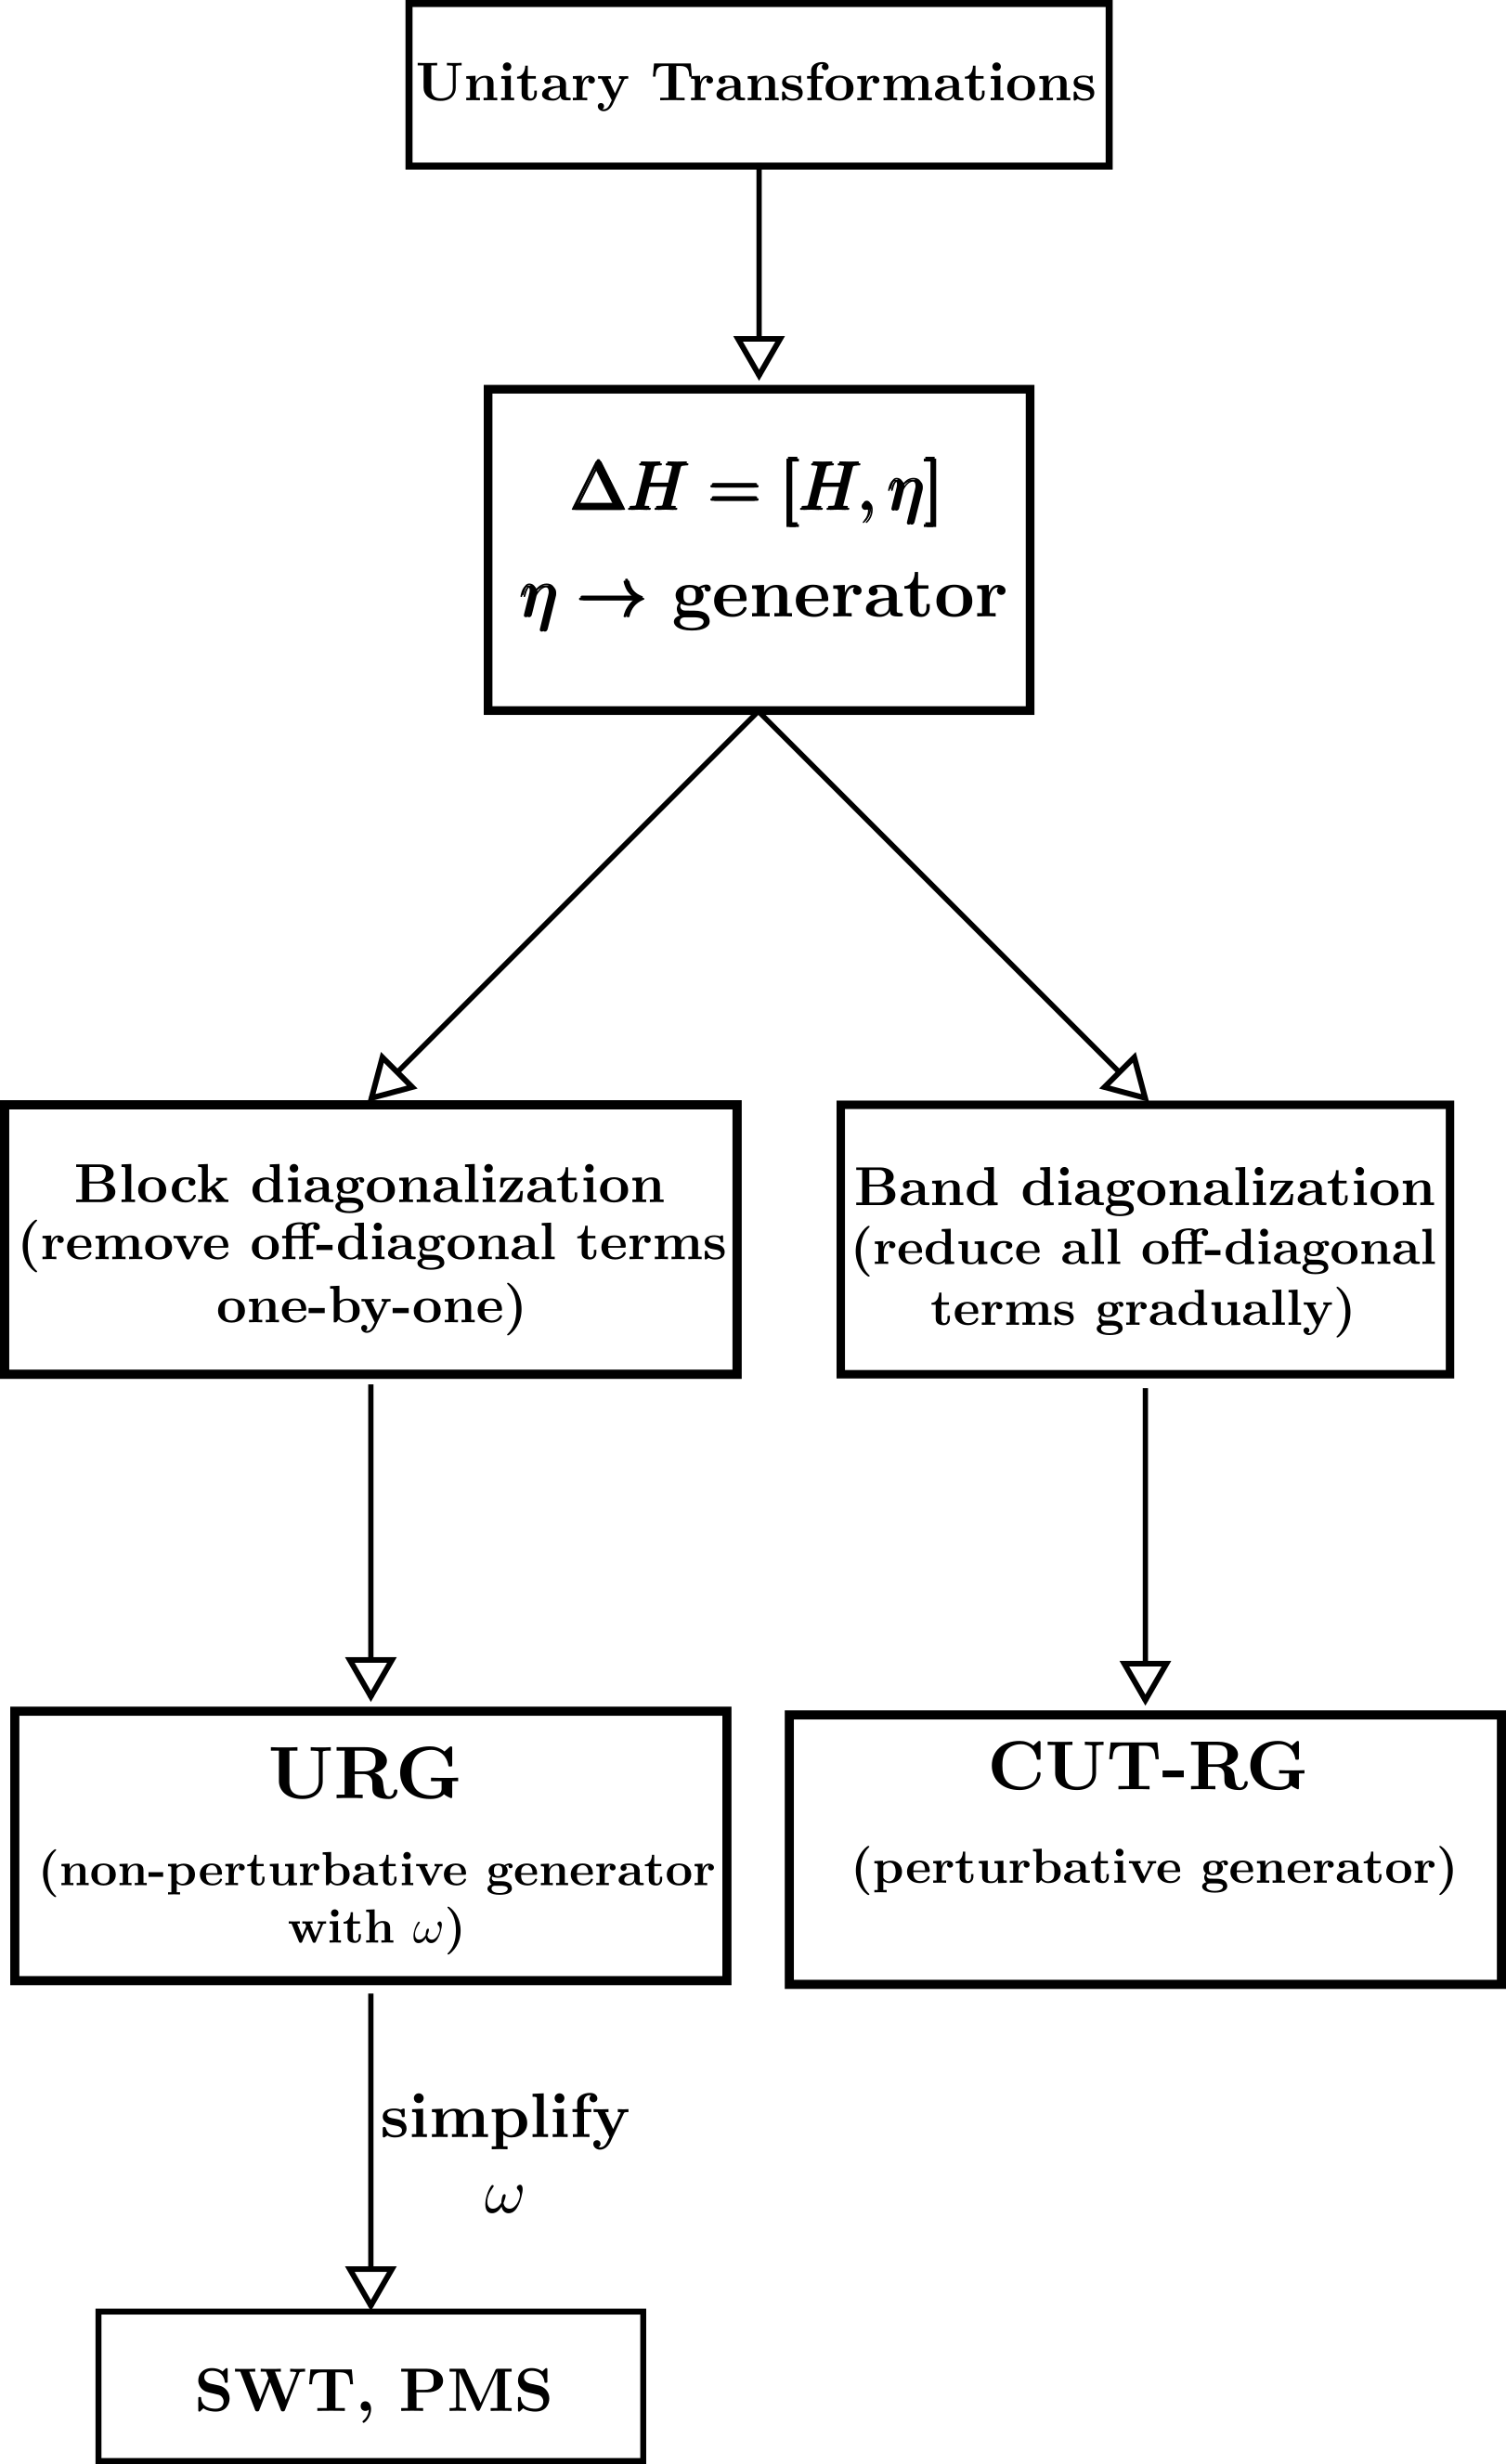
\includegraphics[scale=0.22]{../figures/unitaries.png}
	\captionof{figure}{Comparison of the various unitary transformations and their relationships to each other.}
\end{center}
